% vim:tw=72 sw=2 ft=tex
%         File: thoughts_report.tex
% Date Created: 2013 Jun 18
%  Last Change: 2014 May 22
%       Author: hhiker
\documentclass[a4paper]{book}
\usepackage{pdfpages}
\usepackage{xltxtra}
\usepackage{xcolor}
\usepackage{xeCJK}
\usepackage{minted}
\usepackage{booktabs}
\usepackage{mathtools}
\usepackage{paralist}
\usepackage[colorlinks=true,linkcolor=red]{hyperref}
% \usepackage{hyperref}
\usepackage{varioref}
\usepackage{cleveref}
\newcommand{\head}[1]{\textbf{#1}}
\setCJKmainfont[BoldFont=SimHei,ItalicFont=SimSun]{KaiTi}

\newtheorem{theorem}{Theorem}[section]
\newtheorem{lemma}[theorem]{Lemma}
\newtheorem{proposition}[theorem]{Proposition}
\newtheorem{corollary}[theorem]{Corollary}
\newtheorem{definition}{Definition}[section]
\newtheorem{remark}{Remark}[section]

\newenvironment{proof}[1][Proof]{\begin{trivlist}
\item[\hskip \labelsep {\bfseries #1}]}{\end{trivlist}}
\newenvironment{example}[1][Example]{\begin{trivlist}
\item[\hskip \labelsep {\bfseries #1}]}{\end{trivlist}}

\newcommand{\qed}{\nobreak \ifvmode \relax \else
      \ifdim\lastskip<1.5em \hskip-\lastskip
      \hskip1.5em plus0em minus0.5em \fi \nobreak
      \vrule height0.75em width0.5em depth0.25em\fi}

\DeclareMathOperator*{\argmin}{argmin}
\DeclareMathOperator*{\argmax}{argmax}

\begin{document}
\begin{titlepage}

\newcommand{\HRule}{\rule{\linewidth}{0.5mm}} % Defines a new command for the horizontal lines, change thickness here

\center % Center everything on the page
 
%----------------------------------------------------------------------------------------
% HEADING SECTIONS
%----------------------------------------------------------------------------------------

\textsc{\LARGE University of Science and Technology of China \&\&
  Microsoft Research Asia}\\[1.5cm] % Name of your university/college
\textsc{\Large Graduation Thesis}\\[0.5cm] % Major heading such as course name
\textsc{\large Bachelor of Engineering}\\[0.5cm] % Minor heading such as course title

%----------------------------------------------------------------------------------------
% TITLE SECTION
%----------------------------------------------------------------------------------------

\HRule \\[0.4cm]
{ \huge \bfseries Learning Intermediate Representation of Large Scale
  Corpus}\\[0.4cm] % Title of your document
\HRule \\[1.5cm]
 
%----------------------------------------------------------------------------------------
% AUTHOR SECTION
%----------------------------------------------------------------------------------------

\begin{minipage}{0.4\textwidth}
\begin{flushleft} \large
\emph{Author:}\\
Shuai \textsc{Li} % Your name
\end{flushleft}
\end{minipage}
~
\begin{minipage}{0.4\textwidth}
\begin{flushright} \large
\emph{Supervisor:} \\
Jinhui \textsc{Yuan}\\ % Supervisor's Name
Linli \textsc{Xu} % Supervisor's Name
\end{flushright}
\end{minipage}\\[4cm]

% If you don't want a supervisor, uncomment the two lines below and remove the section above
%\Large \emph{Author:}\\
%John \textsc{Smith}\\[3cm] % Your name

%----------------------------------------------------------------------------------------
% DATE SECTION
%----------------------------------------------------------------------------------------

{\large \today}\\[3cm] % Date, change the \today to a set date if you want to be precise

%----------------------------------------------------------------------------------------
% LOGO SECTION
%----------------------------------------------------------------------------------------

%\includegraphics{Logo}\\[1cm] % Include a department/university logo - this will require the graphicx package
 
%----------------------------------------------------------------------------------------

\vfill % Fill the rest of the page with whitespace

\end{titlepage}
\tableofcontents
\pagebreak
\listoffigures
\listoftables
\pagebreak

\chapter*{Preface}
  Starting from the birth of computer science, scientists are constantly
  undertaking great endeavor to understand natural(human) language.
  Besides being part of the supreme goal to build an aritificial
  intelligence thus gaining more insight into humans themselves, the
  applications of natural language processing(a.k.a NLP) play an
  important role in prompting the advance of this area. Nowadays, also,
  the ever boosting amount of collective knowledge digitalized and
  stored -- in the form of news, blogs, Web pages, scientific articles,
  books, images, sound, video, and social networks -- calls for an
  efficient way to organize, search and understand these vast amount of
  information.

  The approachs to understand natural language evolve from rule based
  ones to statistical model based ones from the origin of this field to
  now. Recently research in this area has increasingly focuses on
  unsupervised and semi-supervised learning algorithms both for its
  intuitively conforming with how human learns and the large amount of
  unlabeled data could be obtained from the World Wide Web. The key idea
  underlying this approach is to find a proper representation of natural
  language, which can capture the hidden semantical information. The
  well-known technique -- deep learning, also falls under this category.
  However, despite the success, such as word
  embedding\cite{DBLP:journals/corr/abs-1103-0398} and its
  implementation word2vec why such a representation is able to capture
  the linguistic features underlying one word and its embedding context
  is still unclear. Neural network is mathematically equivalent to
  fitting data into one nonlinear function, which gives no intuitive
  interpretation.  Understanding natural language is a tough task, so is
  giving an explanation of why word embedding works. We get started by
  verifying simple assumptions. In this context, since the main strength
  of neural network is its capability to capture nonlinear information
  in whatsoever probabilistic space of natural language, we may ask is
  the ability to recognize all kinds of nonlinear features of natural
  language that makes it stands out? This brings forward the question:
  how could we measure nonlinearity?

  Inspired by the theoretical sound probabilistic model in natural
  language -- \textbf{Topic Model}, we tackle this problem in a
  statistical view. Nonlinearity relation between variables means the
  existence of higher order statistic. Therefore, we are going to try
  figuring out whether higher order statistic matters in NL. This idea
  is also motivated by the already made discussion in Computational
  Vision(CV) field. By learning how the comparison is made between
  methods only utilizing second order statistic and the one that
  utilizes higher order statistic in CV, we try to do similar research
  on the statistic of NL. This is what this thesis aims at.

  More formally, this thesis serves the following purposes:
  \begin{itemize}
    \item An almost thorough introduction to algebra and probability
      theory behind machine learning. It stresses on the intuition
      behind and gives rigorous and complete definitions and proofs.
    \item An elaboration on methods to obtain an intermediate
      representation utilizing different order of statistic information
      contained in the context. For example, Principle Component
      Analysis, a.k.a. PCA, only use second-order statistic information
      with the assumption that the distribution should be gaussian while
      Independent Component Analysis, a.k.a. ICA uses higher order
      statistics with non-gaussian assumption.
    \item Illustrate how the problem that whether higher order statistic
      in NL matters can be addressed.
  \end{itemize}

  The thesis is organized as following: Chapter \ref{chp:linear_algebra}
  and Chapter \ref{chp:matrix_calculus} mainly focus on introducing
  relevant mathematical background, but they also explain the first
  technique involved to get intermediate representations -- PCA, in
  great detail. Chapter \ref{chp:probability_theory} introduces
  probability theory, including bayesian probability. Chapter
  \ref{chp:intermediate_representation} describes how the need of an
  exploration of different context statistic is arised by introducing
  recent work on learning intermediate representation. Chapter
  \ref{chp:exploring_different_stat} describes what can we do with
  Natural Languages's statistic and briefly introduces some work done in
  large scale machine learning to tackle with large volumes of data
  needed by learning intermediate representation. Lastly an illustration
  about finding synonym using LSA is showed.

  All square matrices in this book belong to $R^{n \times n}$ and all
  rectangular matrices belong to $R^{m \times n}$ if not explicitly
  described.

\chapter{Linear Algebra}
\label{chp:linear_algebra}

  \section{Singular Value Decomposition}

  Singular Value Decomposition(SVD) can be viewed as a way to obtain an
  intermediate representation. In 19th century, pysicists discovered new types
  of element only by analyzing light spectrum.  What's more, they used light
  spectrum to analysis the compositions of stars billions of light year away. In
  ML field, this intermediate representation is used in community
  detection(spectral graph theory), natural language processing(eigenwords) and
  etc. Singular Value Decomposition can be viewed as an extension of spectral
  decomposition in linear algebra.

  In this chapter, I will use some primer knowledge of \textbf{Singular Value
    Decomposition} as thread to introduce relevant linear algebra knowledge in
  ML.

  \begin{theorem}
  \label{thm:spectral_theory}
  given one matrix $A$, it can be decomposed in the following way:

  \begin{displaymath}
    A = \sigma_{1}
      \begin{pmatrix}
        | \\
        u_{1} \\
        |
      \end{pmatrix}
    \begin{pmatrix}
      - & v_{1}^{T} & - 
    \end{pmatrix}
      + \cdots + \sigma_{r}
      \begin{pmatrix}
        | \\
        u_{r} \\
        |
      \end{pmatrix}
    \begin{pmatrix}
      - & v_{r}^{T} & - 
    \end{pmatrix}
  \end{displaymath}
  where $\sigma_{i}, i = 1, \ldots, r$ is the singular value of $A$,
  $u_{i}, i = 1, \ldots, r$ is the left singular vectors of $A$, and
  $v_{i}, i = 1, \ldots, r$ is the right singular vectors of $A$.
  \end{theorem}

  This is the goal I plan to demysterify in this chapter.

  \begin{figure}[h]
    \begin{center}
      \includegraphics[width=0.65\textwidth]{./figures/light_spectral.jpg}
      \caption{Light Spectral\label{fig:light_spectral}}
    \end{center}
  \end{figure}
  Along with PCA(Principle Component Analysis), introduced in next
  chapter, which is the first application of eigens(short for eigenvalue
  and eigenvector) that causes me to begin to think about eigens'
  nature, they prompted me to determine to understand the math related
  to eigens.  Eigenvalue and eigenvector originate from solving
  mechanical problems\cite{Hawkins19751}, but for people want to work in
  machine learning field, it is its nature in algebra that makes it
  important. I will explain various definition, theorems and
  applications concerning eigens along the way.


  \section{What Does It Mean to Learn Linear Algebra?}

  What does it mean to learn linear algebra? The essense of learning
  is to understand the nature of the target you are going to learn,
  which means let go minutea, and condense compact knowledge, usually
  meaning the intuition behind it. The linear algebra course I learnt
  in my college did this job not very well. Based on my current
  limited understanding, understanding linear algebra well should be
  able to understand the following concepts well:

  \begin{enumerate}
    \item Linear combination, linear dependence and independence
    \item Vector space
    \item Orthogonality
    \item Determinant
    \item Eigenvalue and eigenvector
    \item Linear transformation
  \end{enumerate}

  Abstractly, linear combination, linear dependence and independence
  are ideas crystalized when mathematicians are investigating
  equations, which involves linear, nolinear, differential ones and
  etc. While vector space is one level of abstraction mathematicians
  made to formally describe the world. Orthogonality is one essential
  characteristics of basis of vector space, while determinant is a
  summary, or fingerprint of one matrix, so is eigens. Linear
  transformation is one type of change that is simple but matters.

  To understand spectral decomposition, understand why those six points
  except for determinant are introduced and important is necessary. I
  will leave the discussion of determinant for the time being, since
  understanding its nature may involve another deep water of knowledge
  which I do not have time for them yet. Note that the content following
  is not an explanation of the above concepts one by one but a thread
  gives you a sense why those concepts are important.

  \section{Vector Space}

  I will start with vector space, since linear combination, dependence and
  independence should be a prerequisite if anyone wants to read this.

  Vector space is the starting place where you try to build your
  understanding of your mathematical world. Imagine we just live in
  a 3D world, if using the center of the earth as reference, our
  location is determined by longitude and latitude, since altitude
  does not matter for most of we human are just living on such a
  thin layer on earth. This is a 3D vector space. Our physical world
  exists on such vector space. More academically, taking image space as
  an example, image is represented as a numerical array containing the
  intensity value of its picture elements, or pixel. To make the example
  concrete, say that we are dealing with images of a fixed size of
  256-by-256 pixels. This gives a total of $ 65536 = 256^2 $ pixels in
  an image. Each image can then be considered as a piont in a
  65536-dimensions space, each axis of which specifies the intensity
  value of one pixel\cite{Hyvrinen09}.  The goal of computer vision is
  to discover the rules that forms this vector space.

  The above is the intuition of vector space. The mathematical vector
  space is slightly different from the example above. More formally,
  vector space is an abstraction mathematicans made to model our real
  world, which could be the physical world, or the image space. Formal
  definition of vector space is showed in the following\cite{amann2006analysis}:

  \begin{definition}
    \textbf{Vector Space}: A vector space over the field K (or simply, a
    K-vector space) is a triple (V, +, $\cdot$ ) consisting of a nonempty set
    V, an `inner' operation + on V called \textbf{addition}, and an `outer'
    operation
    \begin{equation*}
      K \times V \rightarrow V, (\lambda, v) \rightarrow \lambda \cdot v
    \end{equation*}
    called \textbf{scalar multiplication} which satisfy the following
    axioms:
    \begin{itemize}
      \item (V, +) is an Abelian group.
      \item The distributive law holds:\\
        $\lambda \cdot (v + w) = \lambda \cdot v + \lambda \cdot w,
        (\lambda + \mu) \cdot u = \lambda \cdot v + \mu \cdot v, \lambda,
        \mu \in K, v, w \in V$
      \item $\lambda \cdot (uv) = (\lambda u) \cdot v, 1 \cdot v = v,
        \lambda, \mu \in K, v \in V.$
    \end{itemize}
  \end{definition}

  This is a rather mathematical definition, which involves a number
  of definitions not mentioned. If you are interested and determined
  as I am, the following sections will introduce the missing
  definitions. If not, the intuition is enough to keep going -- this
  is the condensed knowledge.

  In the following sections trying to explain mathematical vector
  space, I am going to deal with the axiomization of natural number,
  which interprets objects, not only natural number, but also other
  mathematical object, like the whole number system, matrix, and
  etc, as elements in set. Built on set, which is the set theory,
  mathematicians developed algebra. Bit by bit, relevant concepts
  will be explained.

    \subsection{The Folk Story of Mathematics}
    \label{subsec:The Folk Story of Mathematics}

    Here, I may digress a little to describe my understanding about why
    mathematics comes into being one so abstract discipline, the roles
    different areas of mathematics play in the whole stage, and lastly,
    little about matrix.

    Just like the so important data structure in computer science,
    which plays a role to formalize nature into something the computer
    can understand -- stack, queue, tree, heap, etc, there is
    something similar in math world. it is called mathematical object.

    Starting from nature number, mathematicians invented integer,
    rational number, irrational number, which combined into real number,
    imaginary number, which combines with real number to construct the
    whole amazing number theory of modern math. Numbers are just a
    math abstraction of common sense. The nature number one at the
    very beginning was not nothing but means a tent or something else
    concrete. Numbers are mathematical objects.

    Usually, math begins from the concrete, evolves into the abstract
    -- meaning evolving from real-world object into mathematical
    object.  What is a number? There is no formal mathematical answer
    for a very long time in the history. Just like you ask your father
    in your childhood: ``what is a lion?'' The only way to make you
    understand is to bring you to the zoo and point at the lion, and
    say: ``Look, that is a lion!''
    
    But this should not be the case if math wants to keep developing.
    So, during 19th century, mathematicians reconstruct the whole
    number theory, based on set theory, mathematical logic and peano
    theorem. From then on, classical mathematics becomes modern
    mathematics.

    Set theory, number theory, mathematical logic are foundations of
    mathematics. Normally, they do not have any practical usage -- they
    are building blocks of the ones that have practical usage.

    Using those building blocks, mathematicians invented structure of
    them -- group, ring, field. Those are the ultimate abstraction of
    real-world objects. What's more, structures also capture
    calculation(operation and relation) between them -- they are
    captured in the ultimate abstraction form as well.

    Equipped with weapons which has bigger granuity, mathematicians built
    worlds, which are called spaces mathematically. For example, vector
    space is one space who is notoriously famous. Those worlds are stages
    for all kinds of dramas played by mathematical object. Those are
    where applications of math happen.

    From what I have learnt, applications of math are mainly doing two
    kinds of things: 
    
    \begin{itemize}
      \item
        Given real-world stuffs, try to find a world, then try to find
        the stuff's inner mathematical structure in that world. The
        world normally are chosen using two criteria: similarity with
        the real world; low computation complexity.
      \item
        Though finding the world and the structure is aleady a
        notoriously difficult thing, the essential usage of finding
        those two is to predict. The world and structure are publicly
        known mathematical model. The meaning of mathematical model is
        to predict -- predicting the real-world stuff that are not used
        when building the model and predicting how this model will
        evolve.
    \end{itemize}

    The latter brings forward another pillar of math -- the study of
    evolvement. The notorious calculus falls under this category.
    Acutally, a whole branch of math called analysis is doing this kind
    of thing.

    Lastly about the folk story of mathematics, I will talk something
    about matrix. In the highest level of abstraction, it is one kind
    of mathematical object, but it contains a huge amount of
    information in it. This is the tool mathematicians invented to
    combat the complexity of the real world -- one thing in the real
    world contains an enormorous amount of information in themselves as
    well. As will be elaborated later, there are two views about matrix:
    view it as a rectangular array of numbers or representation of
    linear transformation.

    A genius example for this: the movie \textit{the Matrix.}


    \subsection{Axiomization of the intuition -- Peano Axiom}

    Now folk story ends and the mathematical part begins.

    The notion of a natural number is one of the most fundamental and most
    important in mathematics. The system of natural numbers was the first
    abstract scientific concept created by man. Having dealt in everyday
    life, with certain quantitieso of real things, people noted certain
    general properties of numbers and developed the notion of counting
    numbers. This apparently simple concept is in some ways so profound that
    it has prompted some people to believe that this concept comes directly
    from God. A great German number theorist, Leopold Kronecker(1823 - 1891)
    said:``God made the natural numbers, all else is the work of
    man.''[Heinrich Weber. Leopold Kronecker. Jahresberichte DMV 1893;
    2:5-31]. Creating the notion of a natural number is first step not only
    in mathematics, but in the development of all
    sciences\cite{dixon2011algebra}.

    The history is long, however, the modern axiomatic theory of natural
    numbers is developed at the end of the nineteenth century and named in
    honor of a famous Italian mathematician, Giuseppe Peano(1858 - 1932),
    whose input in the axiomatization of natural numbers was of exceptional
    mathematical and philosopical value\cite{dixon2011algebra}.

    \begin{definition}
      \textbf{Peano Axiom}: The set $N_0$ is a nonempty set and for all $ a
      \in N_0 $, there is a uniquely defined element $a'$, called the
      immediate successor of a and for which the following axioms hold:
      \begin{itemize}
        \item
          \textbf{(P 1)}  a = b implies that $a' = b'$.
        \item
          \textbf{(P 2)}  There is an element 0(the natural number 0) such
          that 0 is not the immediate successor of any element of $N_0$.
          Thus $0 \neq a'$ for all elements $ a \in N_0 $.
        \item
          \textbf{(P 3)}  If $a,b \in N_0$ and $ a' = b'$, then $a = b$.
        \item
          \textbf{(P 4)}  (the induction axiom). Let M be a subset of $N_0$
          satisfying the conditions:
          \begin{itemize}
            \item $ 0 \in M$;
            \item if $a \in M$, then $a' \in M$.
          \end{itemize}
          Then $ M = N_0 $.
      \end{itemize}
    \end{definition}

    The natural number is defined as\cite{dixon2011algebra}:

    \begin{displaymath}
      0 = \emptyset, 1 = \{\emptyset\}, 2 = 1 \cup \{1\} = \{0, 1\}, 3 = 2 \cup
      \{2\} = \{0, 1, 2\} ...
    \end{displaymath}

    In the book\cite{dixon2011algebra}, the author does not talk about why
    natural number is defined this way:
    \begin{quote}
      Such a level of exposition is far beyond the scope of this book and
      requires significant mathematical maturity.
    \end{quote}

    I just take those definition as natural abstraction of the counting
    symbol used by people.

    With the Peano Axiom, all normal arithmetical properties can be derived.

    Ok. I think this is where I should stop digging.


    \subsection{Cartesian Product}

    Algebra, and much of math deals with domain and mapping between domains.
    The domain can be natural number, real number, matrix, vector. And the
    mapping belongs to the universal set -- the set of Cartesian product.

    \begin{definition}
      Let $A$ and $B$ be sets. Then the set $A \times B$ of all ordered
      pairs (a, b) where $a \in A, b \in B$ is called the Cartesian product
      of the sets $A$ and $B$.
    \end{definition}

    I first met this concept at the time I leart the Database course.
    But I do not get a intuitive feeling about it that time. Actually,
    the real plane $R^2$ is a natural example of a Cartesian product.
    Cartesian product is like a stage where all algebra players must
    play on such stage.

    \begin{remark}
      The definition and examples are all in two dimension, however,
      Cartesian product can extend to any dimension.
    \end{remark}

    Now, object and their stage have been introduced. Theory of
    mathematics is built on them. To advance further, we may try to
    think what defines our world? There is branch in AI(Artificial
    Intelligence) called ontology, which tries to mathematically define
    the whole phsical world. The main technique it uses is second order
    logic, which describes the world using objects, objects's attributes
    and the operation operated on objects. For example, the
    King(object), with long legs(attributes of object) is on(operation
    between objects) the throne(another object).  Similarly things
    happens in the highly abstracted world of mathematics. Algebra
    mainly deals with algebraic operations between objects(elements of
    sets), properties of algebraic structure. Those operations and
    properties usually define an algebra structure. In following
    sections about algebra, common operations, properties of algebraic
    structures and typical algebra structure will be introduced.

    \subsection{Algebraic Operations}

    With the objects we can manipulate(this part means set theory,
    which is not formally talked about but informally, as we learnt in
    high school, it is just a collection object, whose intuition is
    explained again and again.), and the stage their mappings play
    on(Cartesian product), we may try to establish some theory upon
    them, which is the theory that we are familiar with since young
    age.

    \begin{remark}
      There are no rules existing yet. Object(set) are just object. Mappings
      are just mappings.
    \end{remark}

    We are used to the concept of operations, such as addition,
    subtraction.  They are abtracted from our daily life. As the
    universal theme in mathematical world, mathematicians need to
    generalize them -- they bring forward the idea of binary algebraic
    operations, which is one of the most fundamental in
    mathematics\cite{dixon2011algebra}.

    \begin{definition}
      \textbf{Binary Operation}: Let $M$ be a set. The mapping $\theta:
      M \times M \rightarrow M$ from Cartesian square of $M$ to $M$ is
      called binary(algebraic) operation on set $M$. Thus, corresponding
      to every ordered pair $(a,b)$ of elements, where $a,b \in M$, there
      is a uniquely defined element $\theta(a,b) \in M$. The element
      $\theta(a,b) \in M$ is called composition of the elements a and b
      relative to this operation.\cite{dixon2011algebra}
    \end{definition}

    Then starting from binary algebraic operation, mathematicians build the
    algebraic structure bit by bit.

    \begin{remark}
      There is one important note given about notation in the
      thesis\cite{dixon2011algebra}. It is often rather cumbersome to keep
      referring to the function $\theta$ and using the notation
      $\theta(a,b)$. There are several shorthand symbols that are employed
      and $\theta(a,b)$ is often written using such special notation. For
      example, the operation might be denoted by $\diamond$ and we might
      then write $\theta(a,b) = a \diamond b$. We note that, in general,
      $\theta(a,b)$ will be different from $\theta(b,a)$. However, quite
      often, even the notation $a \diamond b$ is confusing, and most often
      we would rather write the operation $\diamond$ using something more
      familiar. The most familiar binary operators are $+$  and $\cdot$ and
      it is these symbols that are most often useful in writing such
      operations. Thus, instead of writing $a \diamond b$ we may write $a +
      b$ or $ a \cdot b$. It is important to understand that sometimes
      these symbols will have familiar meanings, but not
      always.\cite{dixon2011algebra}
    \end{remark}

    \subsection{Important Properties of Algebraic Structure}

      \subsubsection{Rules}

      \begin{definition}
        \textbf{Commutativity}: A binary operation on a set $M$ is called commutative if $ab = ba$ for
        each pair $a,b$ of elements of $M$.\cite{dixon2011algebra}
      \end{definition}

      \begin{definition}
        \textbf{Associativity}:A binary operation on a set $M$ is called associative if $(ab)c =
        a(bc)$ for each triple $a,b,c$ of elements of
        $M$.\cite{dixon2011algebra}
      \end{definition}

      \subsubsection{Special Elements}

      Besides those two rules, the zero and identity element in one algebraic
      structure are of special status.

      \begin{definition}
        \textbf{Neutral Element}:Let $M$ be a set with binary operation. The
        element $e \in M$ is called a neutral element under this operation if
        $ae = ea = a$ for each element $a$ of the set
        $M$.\cite{dixon2011algebra}
      \end{definition}

      \begin{remark}
        If the operation on $M$ is written multiplicatively, then the term
        \textit{identity element} is usually ued rather than neutral element
        and often $e$ is denoted by $1$ or $1_m$. If we use the additive form,
        then the neutral element is usually called the \textit{zero element}
        and is often denoted by $0_M$, so that the definition of the zero
        element is $ a + 0_M = 0_M + a = a$ for each element $a \in
        M$.\cite{dixon2011algebra}
      \end{remark}

      \subsubsection{Algebraic Properties}

      Properties can also be understanded as restriction put on algebraic
      structure or a abstraction of natural properties of natural algebraic
      structure.

      \begin{definition}
        \textbf{Stable}: Let $M$ be a set with a binary operation. A subset S
        is called stable under this operation if for each pair of elements
        $a,b \in S$ the element ab also belongs to S.\cite{dixon2011algebra}
      \end{definition}

      \begin{definition}
        \textbf{Invertibility}: Let $M$ be a set with binary operation and
        suppose that there is an identity element $e$. The element $x$ is
        called an inverse of the element $a$ if 
        \begin{displaymath}
          ax = xa = e.
        \end{displaymath}
        if $a$ has an inverse then we say that $a$ is invertible.\cite{dixon2011algebra}
      \end{definition}

      \begin{remark}
        Invertibility is just a property. We are used to take it as granted if we
        are so used to the natural operation such as addition or
        multiplication. Some algebraic structure has it, but some do not.
      \end{remark}

    \subsection{Algebraic Structures}

    \begin{definition}
      \textbf{semigroup}: A nonempty set $S$ is called a semigroup if $S$
      has an associative binary operation defined on it. If this operation i
      commutative, we will say that $S$ is a commutative semigroup.\cite{dixon2011algebra}
    \end{definition}

    \begin{definition}
      \textbf{group}: A semigroup $G$ with identity is called a group if
      every element of $G$ is invertible. Thus, a group is a set $G$
      together with a binary algebraic operation $(x,y) \rightarrow xy$
      where $x,y \in G$, such that the following conditions(the group axiom)
      holds:\cite{dixon2011algebra}
      \begin{compactitem}
      \item \textbf{G 1} The operation is associative so that $x(yz) =
        (xy)z$ for all $x,y,z \in G$.
      \item \textbf{G 2} $G$ has an identity element, an element $e$ such
        that $xe = ex = x$ for all $x \in G$; often $1$ or $1_G$ is used in
        place of $e$.
      \item \textbf{G 3} Every element $x \in G$ has an inverse $x^{-1}$
        such that $xx^{-1} = x^{-1}x = e$.
      \end{compactitem}
    \end{definition}

    \begin{definition}
      \textbf{abelian group}: If the group operation is commutative, then
      the group is callled abelian(in honor of the great Norwegian
      mathematician Nielss Henrik Abel(1802 - 1829).\cite{dixon2011algebra}
    \end{definition}

    \subsubsection{Mapping Properties}

    \begin{definition}
      Let $M, S$ be sets with binary operations that we denote by $\ast$ and
      $\diamond$, respectively. Let $ f:M \rightarrow S $ be a mapping. Then
      $f$ is called a homomorphism, if 
      \begin{displaymath}
        f(x\ast y) = f(x) \diamond f(y)
      \end{displaymath}
      for arbitrary elements $x,y \in M$.\cite{dixon2011algebra}
    \end{definition}

    If the mapping $f$ is homomorphism, we say that the mapping $f$
    respects the operations. An injective homomorphism is called
    \textbf{monomorphism}. A surjective homomorphism is called an
    \textbf{epimorphism} and a bijective homomorphism is called an
    \textbf{isomorphism}.\cite{dixon2011algebra}

    When two structures $M,S$ are isomorphic in this way, there is no
    difference between the structures other than the names we give to the
    elements of the two sets $M$ and $S$ and the names $\ast$ and $\diamond$
    that we give to the names of the operators. Other than this, the
    structures of $M$ and $S$ are identical.\cite{dixon2011algebra}

    If $M$ is a set with binary operation, then the study of $M$ has two
    aspects. The first aspect is concerned with the nature of the elements
    and the structure of $M$, while the second one concerns properties of
    the operation. This enables such a study to be conducted from different
    points of view. We can study the relationship between the elements and
    the subsets of $M$ and also study individual properties with repsect to
    given operation. Such an approach is feasible for the study of concrete
    sets, such as permutations, transformations of the plane and space,
    symmetries, matrices, and so on. However, we can conduct a study of the
    properties that does not depend on the nature of the elements and which
    is completely defined by the operation. This approach is the key
    approach in algebra and it can be covered by very efficienty, thanks to
    the fundamental notion of isomorphism. Making this more concrete,
    Gottfired Leibniz(1646 - 1716) introduced the general notion of an
    isomorphic relation(which he called a similarity) and pointed out the
    possibility of the identification of isomorphic operations and
    relations. He brought attention to a classical example of isomorphism,
    namely the mapping $x \rightarrow logx$ from the set of all positive
    real numbers with operation of multiplication to the set of all real
    numbers with the operation of addition. A great French mathematician,
    Evariste Galios(1811 - 1832), was also familiar with the idea of
    isomorphism. He understood the corresponding elements of isomorphic sets
    $M$ and $S$ have the same properties with repsect to the given
    operation. This notion in its general form was developed in the middle
    of the nineteenth century. In abstract algebra, we study only such
    properties that are unchanged by isomorphisms.\cite{dixon2011algebra}

    \subsection{Fields}

    After becoming familiar with basic algebraic structure and their
    properties, I could finally reach the definition of \textbf{Field},
    which is the one used extensively and may be the most famous one
    amoung various algebra structure.

    \begin{definition}
      \textbf{Division Ring}: A set $D$ with two binary algebraic
      operations, addition and multiplication, is called a divsion ring if
      it satisfies the following properties:
      \begin{compactitem}
      \item
        the addition is commutative, so 
        \begin{displaymath}
          x + y = y + x
        \end{displaymath}
        for all elements $x,y \in D$;
      \item
        the addition is associative, so
        \begin{displaymath}
          x + (y + z) = (x + y) + z
        \end{displaymath}
        for all elements $x,y,z \in D$;
      \item
        $D$ has a zero element, $0_D$, an element with the property that 
        \begin{displaymath}
          x + 0_D = 0_D + x = x
        \end{displaymath}
        for all elements $x \in D$.
      \item
        each element $x \in D$ has an additive inverse(the opposite or
        negative element), $-x \in D$, an element with the property that
        \begin{displaymath}
          x + (-x) = 0_D;
        \end{displaymath}
      \item
        the distributive laws hold in $D$, so
        \begin{displaymath}
          x(y + z) = xy + xz and (x + y)z = xz + yz
        \end{displaymath}
        for all elements $x,y,z \in D$;
      \item
        the multiplication is associative, so
        \begin{displaymath}
          x(yz) = (xy)z
        \end{displaymath}
        for all elements $x,y,z \in D$;
      \item
        $D$ has a (multiplicative) identity element, $e \neq 0_D$, and
        element with property that
        \begin{displaymath}
          xe = ex = x
        \end{displaymath}
        for each element $x \in D$.
      \item
        each nonzero element $x \in D$ has a multiplicative inverse(the
        reciprocal), $x^{-1} \in D$, and element with property
        \begin{displaymath}
          xx^{-1} = x^{-1}x = e
        \end{displaymath}
      \end{compactitem}\cite{dixon2011algebra}
    \end{definition}

    \begin{definition}
      \textbf{Field}: A division ring $D$ is called a field, if the
      multiplication of its elements is always commutative. Thus a field has
      the additional property that $xy = yx$ for all elements $x,y \in D$.
    \end{definition}

    \subsection{Summary}
    This section is devoted to explaining the idea of vector space, which
    digs back into \textbf{Peano Theorem} and introduces key players in
    the mathematical world and the stage they play on. To summarize, I
    stress the intuition of \textbf{Natural Number} and introduce a
    series of concepts for finally describing the definition of
    \textbf{Vector Space} put forward at the beginning of this section.
    They are concepts abstracted by mathematicians , used extensively in
    daily life and science, and will be used throughout the remaining
    text.

  \section{Foundamental Theorem of Linear Algebra}

  Now, the intuition behind vector space should be appreciated.  Based
  on that, there are already laws discovered by mathematicians to
  describe some typical vector spaces -- \textbf{Foundamental Theorem of
    Linear Algebra}. In my perspective, this is the point that matters
  after finishing learning a linear algebra course.

    \subsection{Introduction of Matrix}

    The matrix first was just a syntax sugar(shortcut) notation for
    describing an array of equations, which was not introduced on the
    stage untill 1800s\cite{wiki_Matrix_(mathematics)}. More formally,
    matrix first came into being by solving equation array like this:

    \begin{align*}
      \begin{cases}
        a_{11}x_{1} +  \cdots + a_{1n}x_{n} & = b_{1}\\
          \hdotsfor{2}                              \\
        a_{m1}x_{1} +  \cdots + a_{mn}x_{n} & = b_{m}
      \end{cases}
    \end{align*}

    Modern mathematicians use model notation to write above equations in
    following form:
    \begin{displaymath}
      \begin{bmatrix}
        a_{11} & \cdots & a_{1n} \\
        \vdots &        & \vdots \\
        a_{m1} & \cdots & a_{mn} 
      \end{bmatrix}
      \begin{bmatrix}
        x_{1} \\
        \vdots \\
        x_{n} 
      \end{bmatrix}
      =
      \begin{bmatrix}
        b_{1} \\
        \vdots \\
        b_{m} 
      \end{bmatrix}
    \end{displaymath}

    After one more step's abstraction, we have matrix-style notation:

    \begin{equation}
      Ax = b
      \label{eq:matrix_form_linear_equations}
    \end{equation}

    As time passes by, matrix evolves into one type of algebraical
    object. To understand this, we compare it with the already mentioned
    example of natural number. When we are in our young age, we use our
    fingers to aid us to count numbers.  That's what our ancestors did
    when they have not invented the number system.  Then, the number
    system(it has been much more enriched beyond natural number) was
    invented to aid our ancestors to cope with more complex problems
    which five, or more, fingers cannot handle.

    The case for matrix is the same. When the concept of matrix is not
    that formalized like today, mathematician used similar things to
    solving linear equations and do geometric transformations using
    matrices \cite{wiki_Matrix_(mathematics)}. Mathematicians
    abstracts the nature of real-world things, then empowered by the
    abstraction, they can deal with more complex problems.
    Applications of matrices are found in most scientific
    fields\cite{wiki_Matrix_(mathematics)}: In every branch of
    physics, including classical mechanics, optics, electromagnetism,
    quantum mechanics, and quantum electrodynamics, they are used to
    study physical phenomena, such as the motion of rigid bodies. In
    computer graphics, they are used to project a 3-dimensional image
    onto a 2-dimensional screen. In probability theory and statistics,
    stochastic matrices are used to describe sets of probabilities;
    for instance, they are used within the PageRank algorithm that
    ranks the pages in a Google search. More abstractly, the major
    application of matrices is to represent linear transformations, that
    is, generalizations of linear functions such as $f(x) = 4x$. For
    example, the rotation of vectors in three dimensional space is a
    linear transformation. If $R$ is a rotation matrix and $v$ is a
    column vector (a matrix with only one column) describing the
    position of a point in space, the product $Rv$ is a column vector
    describing the position of that point after a rotation. The product
    of two matrices is a matrix that represents the composition of two
    linear transformations. Another application of matrices is in the
    solution of a system of linear equations. If the matrix is square,
    it is possible to deduce some of its properties by computing its
    determinant. For example, a square matrix has an inverse if and only
    if its determinant is not zero.\cite{wiki_Matrix_(mathematics)}

    To summarize, matrix has been regarded as two different concepts'
    abstraction:

    \begin{itemize}
      \item compactly represents a linear transformation;
      \item compactly represents an array of numbers;
    \end{itemize}

    More specifically, a matrix $A \in R^{N\times N}$ can be thought of as a
    linear transformation from $C^n$ into $C^n$, but it is also useful to
    think of it as a compact object which represents an array of many
    numbers. The interplay between these two concepts of A, and what the
    array of numbers tells us about the linear transformation, is a central
    theme of matrix analysis and a key to applications\cite{horn2012matrix}.

    \subsection{Four Fundamental Subspaces of Linear Algebra}

    As mentioned in section \ref{subsec:The Folk Story of Mathematics},
    matrix is invented to combat the complexity of real world's objects,
    which encaptures a great amount of information. Those information
    delves in the real world. One major part of ML reseachers' job is to
    assume a vector space, trying to embed real-world information in
    that space, then discovering laws about those information under such
    assumption.

    There are four spaces in equation
    \ref{eq:matrix_form_linear_equations}, which are ``Four Fundamental
    Subspaces'' of linear algebra:
    \textbf{
    \begin{enumerate}
      \item Column Space
      \item Row Space
      \item Null Space
      \item Left Null Space
    \end{enumerate}
    }

    Those four subspaces lift the understanding of $Ax = b$ to a higher
    level -- a subspace level. $A, x$ and $b$ is not just a notation for
    notation simplicity, but reveals some important characteristics of
    the space they delve in. More explanation will be made later.

    Before introducing the four subspaces, we may introduce what is
    subspace\cite{strang2009introduction}.

    \begin{definition}
      A \textbf{subspace} of a vector is a set of vectors (including
      $0$) that satisfies two requirement: \textbf{If $v$ and $w$ are
        vectors in the subspace and $c$ is any scalar, then}:
      \begin{enumerate}
        \item $v + w$ is in the subspace.
        \item $cv$ is in the subspace.
      \end{enumerate}
    \end{definition}

    in other words, the set of vectors is ``closed'' under addition $v +
    w$ and multiplication $cv$ (and $cw$).

      \subsubsection{Column Space \& Row Space}
      To introduce \textbf{Column Space}, we rewrite equation
      \ref{eq:matrix_form_linear_equations} in the following form:

      \begin{displaymath}
        \begin{bmatrix}
          a_{11} \\
          \vdots \\
          a_{m1}
        \end{bmatrix}
        x_{1} + \cdots + 
        \begin{bmatrix}
          a_{1n} \\
          \vdots \\
          a_{mn}
        \end{bmatrix}
        x_{n}
        = 
        \begin{bmatrix}
          b_{1} \\
          \vdots \\
          b_{m}
        \end{bmatrix}
      \end{displaymath}

      This form views linear equations as linear combination of columns
      of matrix $A$. The equation is asking for \textbf{a combination
        that produces $b$}. The space spanned by all combinations of
      columns of $A$ is called \textbf{Column Space} of $A$. Similarly,
      \textbf{Row Space} is the space spanned by all combinations of
      rows of $A$.

      \subsubsection{Null Space \& Left Null Space}
      To introduce \textbf{Null Space}, we replace $b$ with $0$ in equation
      \ref{eq:matrix_form_linear_equations}:

      \begin{equation}
        Ax = 0
        \label{eq:matrix_form_null_linear_equations}
      \end{equation}

      Then, as we do before, we rewrite
      \ref{eq:matrix_form_null_linear_equations} in the form of
      combination of columns of A:

      \begin{displaymath}
        \begin{bmatrix}
          a_{11} \\
          \vdots \\
          a_{m1}
        \end{bmatrix}
        x_{1} + \cdots + 
        \begin{bmatrix}
          a_{1n} \\
          \vdots \\
          a_{mn}
        \end{bmatrix}
        x_{n}
        = 
        \begin{bmatrix}
          0 \\
          \vdots \\
          0
        \end{bmatrix}
      \end{displaymath}

      Equation \ref{eq:matrix_form_linear_equations} is asking for a
      combination of columns of $A$ that makes $b$ (we assume that in
      this case, $b$ will not be $0$), while equation
      \ref{eq:matrix_form_null_linear_equations} is asking for a
      combination that makes $0$, which means columns of $A$ is linear
      dependent, if $x$ is not $0$. Solutions $x$ satisfies equation
      \ref{eq:matrix_form_null_linear_equations} also span a subspace.
      Proof will be omitted. \textbf{Left Null Space} is the null space
      of $A^{T}$. The name left null space comes from taking transpose
      of equation \ref{eq:matrix_form_null_linear_equations}:

      \begin{displaymath}
        x^{T}A^{T} = 0
      \end{displaymath}

      The subspace spans by all combination of solutions $x^{T}$ is
      \textbf{Left Null Space} because $x^{T}$ is on the left of the
      left part of the equation.

    \subsection{Fundamental Theorem of Linear
      Algebra\cite{gilbert_strang_foundamental_theorem_of_linear_algebra}}
    \label{subsec:Fundamental Theorem of Linear Algebra}

    Finally, we reach the \textbf{Foundamental Theorem of Linear
      Algebra}. It connects various important concepts in linear
    algebra.

    \begin{theorem}
      \textbf{Fundamental Theorem of Linear Algebra}:\\
      \textbf{Part One}: Given a matrix $A \in R^{m \times n}$, the
      column space and row space have equal dimension $r$, which equals
      the rank of the matrix $r(A)$. The nullspace $N(A)$ has dimension
      $n - r$, $N(A^{T})$ has dimension $m - r$.
    \end{theorem}

    \begin{proof}

      \textit{NOTE: This proof only points out the key intuitions of the
      rigid proof.}

      Through elimination(normally Gaussian Elimination), every matrix
      can reduce to a form called reduced echelon form, which is an upper
      triangle matrix. The nonzero numbers on the diagonal are called
      pivots of the matrix. The number of pivots is actually the rank ,
      also the dimension of the column space and row space of the upper
      triangle matrix. Since during elimination all operations are
      linear transformation, meaning the space of spanned by the basis
      of the matrix is not changed, which means the rank is not changed.
      Therefore, column space and row space have equal dimension.

      As for the dimension of Null Space, matrix has null space as long
      as columns of matrix $A$ is linear dependent. The number of
      redundant columns is actually the dimension of the null space.
      Similar things happen to left null space.
    \end{proof}

    \begin{theorem}
      \textbf{Fundamental Theorem of Linear Algebra}:\\
      \textbf{Part Two}:
      \begin{itemize}
        \item  $C(A^{T}) = N(A)^{\bot}$, meaning row space and null space are
               orthogonal complements in $R^{n}$
        \item  $C(A) = N(A^{T})^{\bot}$, meaning column space and left null space
               are orthogonal complements in $R^{m}$
      \end{itemize}
    \end{theorem}

    \begin{proof}
      I only explain the intuition for the first one. Rewrite equation
      \ref{eq:matrix_form_null_linear_equations} in the following form:

      \begin{displaymath}
        \begin{bmatrix}
          a_{11} & \cdots & a_{1n} \\
          \vdots &        & \vdots \\
          a_{m1} & \cdots & a_{mn} 
        \end{bmatrix}
        \begin{bmatrix}
          x_{1} \\
          \vdots \\
          x_{n} 
        \end{bmatrix}
        =
        \begin{bmatrix}
          0 \\
          \vdots \\
          0 
        \end{bmatrix}
      \end{displaymath}

      Each row of $A$ is orthogonal to $x$ which is in null space of $A$
      and each row of $A$ and each $x$ belong to $R^{m}$
    \end{proof}


    \begin{theorem}
      \textbf{Fundamental Theorem of Linear Algebra}:\\
      \textbf{Part Three}:
      \begin{displaymath}
        AV = A
        \begin{bmatrix}
            |   &    &   |   &    &   |  \\
          v_{1} & .. & v_{r} & .. & v_{n}\\
            |   &    &   |   &    &   |
        \end{bmatrix}
        =
        \begin{bmatrix}
            |   &    &   |   &    &   |  \\
          u_{1} & .. & u_{r} & .. & u_{m}\\
            |   &    &   |   &    &   |  
        \end{bmatrix}
        \begin{bmatrix}
          \sigma_{1}  &         &       &    &      \\
                      & \ddots  &       &    &      \\
                      &         & \sigma_{r} &    & \\
                      &         &            &    & \\
        \end{bmatrix}
        = U\Sigma
      \end{displaymath}

      Where for $i \in \{1, \ldots , n\}$, the $v_i$ are orthonormal eigenvectors
      of $A^{T}A$, with eigenvalue $\sigma_{i}^{2} \geq 0$. The
      eigenvector matrix diagonalizes $A^{T}A =
      (V\Sigma^{T}U^{T})(U\Sigma V^{T}) = V(\Sigma^{T}\Sigma)V^{T}$.
      Similarly, $U$ diagonalizes $AA^{T}$.
    \end{theorem}

    We can rewrite the above matrix equation in the form of, since V
    will be invertable(explanation will be made later):

    \begin{equation}
      AV = U\Sigma
      A = U\Sigma V^{T}
      \label{eq:singular_value_decomposition}
    \end{equation}

    This is called \textbf{SVD(Singular Value Decomposition)} of matrix $A$,
    where $A$ could be any form of matrix. SVD is the essential operation
    used in PCA.

    Part three of the Fundamental Theorem creates orthogonal bases for
    the four subspaces. More than that, the matrix is diagonal with
    respect to those bases $u_{1}, ... , u_{n}$ and $v_{1}, ... ,
    v_{n}$. However, there is much more math in this part of the
    Fundamental Theorem of Linear Algebra, which involves another major
    part of linear algebra -- eigenvalue and eigenvector. Proof of this
    part will be made after introducing relevant knowledge about eigens.

  \section{Eigenvalue and Eigenvector}

  We touch the idea of eigens because it is used in SVD. Actually, this
  is the way that I gradually understood eigens. One of the concept that
  confuses me the most while I am learning linear algebra and matrix
  calculus is eigenvalue and eigenvector. I was always asking
  \textit{what is the essence of eigenvalue}? Why after such complex
  computation, we decide that such a number and a vector are important.

  In the following pages, the main effort will focus on clarify all kinds
  of definitions and theorems concerning eigenvalue and eigenvector of
  matrix, while trying to give some intuition explanation of why
  eigenvalue and eigenvector are introduced.

    \subsection{Definition}

    To understand eigenvalue, we view matrix as linear transformation.
    Almost all vectors change direction, when they are multiplied by
    $A$.  Certain exceptional vectors $x$ are in the same direction as
    $Ax$. Those are the ``eigenvectors''. Multiply an eigenvector by
    $A$, and the vecotr $Ax$ is a number $\lambda$ times the original
    $x$\cite{strang2009introduction}. The prefix eigen- is adopted from
    the German word eigen for "self-" or "unique to", "peculiar to", or
    "belonging to" in the sense of "idiosyncratic" in relation to the
    originating matrix\cite{wiki_eigens}.

    More mathematically, given a matrix $A$, if a vector satisfies the
    following equation:

    \begin{equation*}
      Ax = \lambda x
    \end{equation*}

    Then, the vector is called the eigenvector $x$ of the matrix $A$,
    and the scalar number $\lambda$ is the eigenvalue of the matrix $A$.
    Eigenvalues and eigenvectors provide insight into the geometry of
    linear transformations.

    \subsection{Essence of Eigenvalue and Eigenvector}

    This definition is weird, at least for me at the first time I learnt the
    concept of it. Much of the reason may be you have to do rather complex
    computation to obtain one matrix's eigenvalues and eigenvectors. I will
    skip the detail computation example here. You can easily find one on
    normal linear algebra textbooks, here\cite{strang2009introduction} is a
    nice book.

    I was always wondering, why and how mathematicians chose and dicover
    such a thing to represent the characteristics of matrix? From my current
    point of view, current higher education about math omitted a major part
    which should be taught -- the historical development of the important
    mathematical concepts. I know this part is hard to teach, because it
    involves a great amount of knowledge. As for the eigenvalue case,
    its development is a long story that spans more than one century.
    There is a similarly important and complex concept called
    determinant in linear algebra. Those two are intertwined together.
    For now, we just focus on eigens.

      \subsubsection{Origin of Eigenvalue}

      At the very beginning, eigenvalue is invented when mathematicians
      were trying to solve mechanics problem. In reflecting upon the
      achievement of the 18th century, d'Alembert wrote in the
      \textit{Encyclopedie} of a transition from the 17th-century age of
      mathematics to the 18th-century age of mechanics. Certainly he was
      correct in the sense that some of the greatest achievement of the
      18th-century geometers involved the application of the new
      analysis of the 17th century to various problems in terrestial and
      celestial mechanics. Furthermore new ideas and devices originated
      from or were inspired by, mechanical problem. This is the case
      with spectral decomposition, its orignins are to be found in the analysis
      of various mechanical problems which involved consideration of an
      algebraic eigenvalue problem. Since the solution of mechanical
      problems was the primary objective, the mathematics remained
      ancillary, but the physical theory compelled the 18th-century
      geometers to concern themselves with mathematical questions about
      the nature of eigenvalue.\cite{Hawkins19751} If you do not satisfy
      with only knowing a fuzzy description, more information can be
      found in the reference\cite{Hawkins19751}.

      \subsubsection{Dynamic Problem}

      Eigenvalues have their greatest importance in \textit{dynamic
        problems}\cite{strang2009introduction}. The mechanical problem
      mentioned previously is one type of dynamic problem. In
      Strang's book\cite{strang2009introduction}, the author uses makov
      matrix as an example to explain how eigenvalue can find steady or
      in another word, static phenomenon in dynamic problem, which
      consequently can simplify, or make unsolvable problems solvable.
      You can find more detail in the book.

      \subsubsection{Discussion: Nature of Eigens}

      I guess there may not be some ultimate nature of eigenvalue and
      eigenvector. The argument is mostly based on it is invented when
      solving relevant problems. The most suitable way to understant it
      may be trying to get to know different important applications it
      can bring to modern science. At least it is the way I began to
      understand.  Eigenvalue can be viewed as a way to characterize
      matrix.  Mathematicians gradually discoverd it by spectral decomposition,
      PCA(introduced next chapter), solving dynamic problem, similar
      matrix and etc.


      \subsection{Real Symmetric Matrix}

      SVD is the application of one type of important matrices --
      symmetric matrix. It is no exaggeration to say that these are the
      most important matrices the world will ever see -- in the theory
      of linear algebra and also in the
      applications\cite{strang2009introduction}. Why any matrix $A$ can
      be decomposed into the form $U\Sigma V$? This is the question
      symmetric matrix should answer.

      \begin{definition}
        A matrix $A$ is symmetric if $A = A'$.
      \end{definition}

      \textit{NOTE: the symmetric matrix here could be matrix with
        imaginary entries as well -- the theorems will be introduced
        below hold as well, however, the definition will be changed as
        this: $A = A^{*}$, where $A^{*} =
        (\bar{A})^T$\cite{wiki_conjugate_transpose}. It is called
        conjugate transpose of A. In this book, we assume all entries of
        matrix are real.}

      Symmetric matrice have special properties that make it
      special\cite{strang2009introduction}\cite{richard_some_basic_matrix_theorems}:

      \begin{enumerate}
        \item The eigenvalues of symmetric matrices are \textbf{real}.
        \item The \textbf{eigenvectors} can be chosen orthonormal with
          each other.
          \begin{enumerate}
            \item The eigenvectors of a symmetric matrix $A$
              corresponding to different eigenvalues are orthogonal to
              each other.
            \item If $\lambda_{i}$ is a repeated root with multiplicity
              $M \geq 2$, then there exist $m$ orthonormal eigenvectors
              corresponding to $\lambda_{i}$.
          \end{enumerate}
      \end{enumerate}

      I will prove those properties later. Now, with those properties,
      let's see what we can do with one matrix $A$.

      First, we see matrix $A \in R^{n \times n}$ with $n$ different
      eigenvalues $\lambda_{1}, ... , \lambda_{n}$, meaning we have:

      \begin{align*}
        Ax_{1} & =  \lambda_{1}x_{1}\\
        \vdots  \\
        Ax_{n} & =  \lambda_{n}x_{n}
      \end{align*}

      Rewrite it in the following form:

      \begin{displaymath}
        A
        \begin{bmatrix}
           |    &         &   |   \\
          x_{1} & \cdots  & x_{n} \\
           |    &         &   |   
        \end{bmatrix}
        =
        \begin{bmatrix}
           |    &         &   |   \\
          x_{1} & \cdots & x_{n} \\
           |    &         &   |   
        \end{bmatrix}
        \begin{bmatrix}
          \lambda_{1} &         &             \\
                      & \ddots  &             \\
                      &         & \lambda_{n} 
        \end{bmatrix}
      \end{displaymath}

      Further rewrite it in the form of only matrix:

      \begin{equation}
        AX = X\Sigma
        \label{eq:matrix_eigens}
      \end{equation}

      With the second properties, columns of $X$, eigenvectors of $X$,
      can be chosen orthonormal, which means we can choose $x_{i}, i \in
      \{1, ..., n\}$ satisfying:

      \begin{displaymath}
        x_{i}^{T}x_{j} = 
        \begin{cases}
          1  & i = j\\
          0  & i \neq j
        \end{cases}
      \end{displaymath}

      This implies $XX^{T} = I$. $X$ is orthogonal with $X^{T}$ and is
      the inverse matrix to $X^{T}$. Further derive
      \ref{eq:matrix_eigens}:

      \begin{align*}
        AX & = X\Sigma\\
        A  & = X\Sigma X^{-1}\\
        A  & = X\Sigma X^{T}
      \end{align*}

      which means $A$ can be decomposed into the form $X\Sigma X^{T}$,
      where $X$'s columns are eigenvectors of $A$ and $\Sigma$ is
      diagonal matrix with eigenvalues of $A$ on its diagonal.

      Here, we are discovering a family of matrices: similar matrices!
      Remember that left multiply an inversible matrix means row
      transformation, while righ multiply an inversible matrix means
      column transformation, which means that if matrix $A$ is a matrix
      originating from a diagonal matrix with eigenvalues $\lambda_{1},
      \cdots, \lambda_{n}$ by some row transformation and column
      transformation. Actually they are called orthogonal
      transformation, which will be introduced in section
      \ref{sec:orthogonal_transformation}. No matter what transformation
      is made, their eigenvalues are the same. Is this interesting?
      Mathematicians's work is to discover shared characteristics among
      seems unrelated objects. Now we bring forward the formal
      definition of \textbf{similar matrix}:

      \begin{definition}
        If two matrices $A$ and $B$ satisfies $A = PBP^{-1}$, where $P$
        is nonsingular(inversible) matrix, then matrix $A$ is a similar
        matrix with $B$, vice versa.
      \end{definition}

      \subsection{Spectral Decomposition}
      \label{sec:spectral_decomposition}
      Note that for any real symmetric matirx $A$, it can be decomposed into
      $X\Sigma X^{T}$, where columns of $X$ are $A$'s eigenvectors. Make a step
      further derivation, we can obtain the spectral decomposition in linear
      algebra.

      \begin{theorem}
        Given any real symmetric matrix, it can decomposed into the form:
          \begin{displaymath}
            A = \sum\limits^{n}_{i=1}\lambda_{i}x_{i}x_{i}^{T}
          \end{displaymath}
      \end{theorem}


      \subsection{Singular Value Decomposition Revisit}

      You may wonder in real-world application, or more specifically, ML
      application, where normally one row of a matrix means one sample,
      and the number of columns are features of the samples, the number
      of rows is always not equal to the one of columns. Why symmetric
      matrices are important, since there are so few of them?

      This is where Singular Value Decomposition stands out. Remember in
      section \ref{subsec:Fundamental Theorem of Linear Algebra}, based
      on equation \ref{eq:singular_value_decomposition}, any matrix can
      be decomposed in similar way. We rewrite it here for clarity:

      \begin{displaymath}
        AV = A
        \begin{bmatrix}
            |   &    &   |   &    &   |  \\
          v_{1} & .. & v_{r} & .. & v_{n}\\
            |   &    &   |   &    &   |  
        \end{bmatrix}
        =
        \begin{bmatrix}
            |   &    &   |   &    &   |  \\
          u_{1} & .. & u_{r} & .. & u_{m}\\
            |   &    &   |   &    &   |  
        \end{bmatrix}
        \begin{bmatrix}
          \sigma_{1}  &         &       &    &      \\
                      & \ddots  &       &    &      \\
                      &         & \sigma_{r} &    & \\
                      &         &            &    & 
        \end{bmatrix}
        = U\Sigma
      \end{displaymath}

      Where for $i \in \{1, \ldots , n\}$, the $v_i$ are orthonormal eigenvectors
      of $A^{T}A$, with eigenvalue $\sigma_{i}^{2} \geq 0$. The
      eigenvector matrix diagonalizes $A^{T}A =
      (V\Sigma^{T}U^{T})(U\Sigma V^{T}) = V(\Sigma^{T}\Sigma)V^{T}$.
      Similarly, $U$ diagonalizes $AA^{T}$. Here I may further note that
      eigenvectors with subscripts bigger than $r$ is eigenvectors of
      eigenvalue zero, which is in the null space of the matrix.

      Although $A$ is not symmetric, $AA^{T}$ and $A^{T}A$ are! Now, we
      going to prove SVD\cite{strang2009introduction}.

      \begin{proof}
        We start at what we have. Since $A^{T}A$ is symmetric matrix, it
        has orthonormal eigenvectors $v_{i}, i \in \{1, ..., n\}$:

        \begin{align*}
          A^{T}Av_{i} = \lambda_{i}v_{i}    
            && \\
          A^{T}Av_{i} = \sigma_{i}^{2}v_{i} 
            && \text{let }\sigma_{i}^{2} = \lambda_{i}\\
          AA^{T}Av_{i} = \sigma_{i}^{2}Av_{i} 
            && \text{Left multiply $A$ for both sides}
        \end{align*}

        We can see that $Av_{i}$ is an eigenvector of $AA^{T}$, and
        $\sigma_{i}^{2}$ is an eigenvalue of $AA^{T}$ which means as long as
        $\sigma_{i}^{2}$ is an eigenvalue of $A^{T}A$, it is an eigenvalue
        of $AA^{T}$. $AA^{T}$ and $A^{T}A$ have the same set of
        eigenvalues.

        What's more, $Av_{i}$ is proportional to $u_{i}$.  To prove SVD,
        we only need to prove:

        \begin{equation}
          Av_{i} = \sigma_{i}u_{i}
          \label{eq:svd_prove_prove_target}
        \end{equation}

        Then, rewrite it in matrix form, we could have:
        \begin{displaymath}
          AV = U\Sigma^{m \times n}
        \end{displaymath}

        where
        \begin{displaymath}
          \Sigma^{m \times n}
          = 
          \begin{bmatrix}
            \sigma_{1}  &         & \\
                        & \ddots  & \\
                        &         & \sigma_{r} &    \\
                        &         &            & 0  &\\
                        &         &            &    & \ddots  & \\
          \end{bmatrix}
        \end{displaymath}

        Here, I explicitly write out the dimension of matrix $\Sigma$
        for clarity.

        Now, we prove equation \ref{eq:svd_prove_prove_target}:

        \begin{align*}
          A^{T}Av_{i} = \sigma_{i}^{2}v_{i}    
            && \\
          v_{i}^{T}A^{T}Av_{i} = \sigma_{i^{2}}v_{i}^{T}v_{i}    
            && \text{Left multiply $v_{i}^{T}$ for both sides}\\
          || Av_{i} ||^{2} = \sigma_{i}^{2}|| v_{i} ||^{2}    
            && \\
          || Av_{i} ||^{2} = \sigma_{i}^{2}    
            && || v_{i} ||^{2} = 1
        \end{align*}

        Since $Av_{i}$ is proportional to $u_{i}$, while the 2-norm(length) of
        $u_{i}$ is $1$ and $Av_{i}$ is $\sigma_{i}^{2}$, the proportion
        is $\sigma_{i}$!

        Proof is done. One last note is that there is a terminology
        called \textbf{economy sized SVD, or thin SVD}, which removes
        the last $m - r$ rows and $n -r$ columns of the right three
        matrices, since in $\Sigma^{m \times n}$, those rows and columns
        are zero, meaning they does not contribute to the final $A$.

        Lastly, besides the matrix equation $AV = U\Sigma$ we get, I
        list two anxillary ones below:

        \begin{align*}
          A^{T}A &= V(\Sigma^{m \times n})^{T}U^{T}U\Sigma^{m \times n} V^{T} = V\Sigma^{n \times n}V^{T}\\
          AA^{T} &= U\Sigma^{m \times n} V^{T}V(\Sigma^{m \times n})^{T}U^{T} = U\Sigma^{m \times m}U^{T}
        \end{align*}

        where
        \begin{displaymath}
          \Sigma^{n \times n}
          = 
          \begin{bmatrix}
            \sigma_{1}^{2}  &         & \\
                            & \ddots  & \\
                            &         & \sigma_{r}^{2} &    \\
                                &         &            & 0  &\\
                                &         &            &    & \ddots  & \\
                                &         &            &    &         &  0 \\
          \end{bmatrix}
          \Sigma^{m \times m}
          = 
          \begin{bmatrix}
            \sigma_{1}^{2}  &         & \\
                            & \ddots  & \\
                            &         & \sigma_{r}^{2} &    \\
                                &         &            & 0  &\\
                                &         &            &    & \ddots  & \\
                                &         &            &    &         &  0 \\
          \end{bmatrix}
        \end{displaymath}

        $r$ is the rank of $A^{T}A$ and $AA^{T}$.
      \end{proof}
Finally, we give explain what is \textbf{singular vectors} and
      \textbf{singular values}:

      \begin{itemize}
        \item Matrix $A$'s \textbf{Singular Values} are $\sigma_{i}, i =
          1, ..., r$, which are the eigenvalues of $AA^{T}$ and
          $A^{T}A$.
        \item Matrix $A$'s \textbf{Left Singular Vectors} are columns of
          $U$, which is eigenvectors of $AA^{T}$, while \textbf{Right
            Singular Vectors} are columns of $V$, which is eigenvectors
          of $A^{T}A$.
      \end{itemize}

      \subsection{Theorems of Symmetric Matrices}

      We have proved SVD in previous section, however, I omitted the
      proofs of relevant theorems of symmetric matrices.
      Proofs\cite{richard_some_basic_matrix_theorems} will be made in
      this section. All entries of matrix is assumed real.

      \begin{theorem}
        The eigenvalues of symmetric matrices are \textbf{real}.
      \end{theorem}

      \begin{proof}
        Assume that $A$ is a symmetric matrix, $\lambda$ is one of
        its eigenvalue and $x$ is one of its eigenvectors. So, we have:

        \begin{align*}
          Ax        &= \lambda x
            && \text{Eigens definition}                 \\
          A\bar{x}  &= \bar{\lambda} \bar{x}  
            && \text{Taking conjugates for both sides}  \\
          \bar{x}^{T}A  &= \bar{\lambda} \bar{x}^{T}  
            && \text{Taking transpose for both sides}   \\
          \bar{x}^{T}Ax  &= \bar{\lambda} \bar{x}^{T}x  
            && \text{Right multiply x for both sides}   \\
          \bar{x}^{T}Ax  &= \bar{\lambda} || x ||^{2}  
            &&
        \end{align*}

        From another perspective, we have:

        \begin{align*}
          Ax        &= \lambda x
            && \text{Eigens definition}                           \\
          \bar{x}^{T}Ax        &= \lambda \bar{x}^{T}x
            && \text{Left multiply $\bar{x}^{T}$ for both sides}  \\
          \bar{x}^{T}Ax  &= \lambda || x ||^{2}  
            &&
        \end{align*}

        So, $\lambda = \bar{\lambda}$, which means $\lambda$ is real.
      \end{proof}

      \begin{theorem}
        The \textbf{eigenvectors} can be chosen orthonormal with each
        other.
        \begin{enumerate}
          \item The eigenvectors of a symmetric matrix $A$
            corresponding to different eigenvalues are orthogonal to
            each other.
          \item If $\lambda_{i}$ is a repeated root with multiplicity
            $M \geq 2$, then there exist $m$ orthonormal eigenvectors
            corresponding to $\lambda_{i}$.
        \end{enumerate}
      \end{theorem}

      \begin{proof}
        Suppose there are two different eigenvalues $\lambda',
        \lambda'$, whose corresponding eigenvectors are $x, y$.

        Based on eigens' definition, we have:
        \begin{align*}
          Ay      &= \lambda'y  
            &&                                          \\
          y^{T}A  &= \lambda'y^{T}  
            && \text{Taking transpose on both sides.}   \\
          y^{T}Ax  &= \lambda'y^{T}x  
            && \text{Right multiply $x$ on both sides.} \\
        \end{align*}

        From another perspective, we have:
        \begin{align*}
          Ax      &= \lambda x 
            &&                                              \\
          y^{T}Ax &= \lambda y^{T}x 
            && \text{Left multiply $y^{T}$ for both sides.}
        \end{align*}

        Since $\lambda$ and $\lambda'$ is different, $y^{T}x$ must be
        zero, which means $y$ and $x$ are orthogonal. As long as we
        normalize them into unit vector, they are orthonormal.

        Now, consider the case when eigenvalues with multiplicity $m \geq
        2$. The main idea behind this
        proof\cite{richard_some_basic_matrix_theorems} is to extract
        orthonormal basis from the eigenvalue with greater than one
        multiplicity untill its multiplicity becomes one. During the
        extraction process, eigenvalues does not change. Thus, at the
        time all eigenvalues have multiplicity one, a set of orthonormal
        basis can be obtained from current matrix. Combining it with
        orthonormal basis extracted, we can have orthonormal basis
        consisting of eigenvectors of original matrix.

        Suppose $\lambda_{i}$ have multiplicity greater than one, it
        must have at least one eigenvector. We denote it as $x_{i}$. For
        any arbitrary nonzero vector $x_{i}$, one can always find an
        additional $n - 1$ vectors $y_{j}, j = 2, ..., n$, so that
        $x_{i}$, together with the $n - 1$ y-vectors forms an
        orthonormal basis. Collect the y vectors in a matrix $Y$, i.e.,
        \begin{displaymath}
          Y = [y_{2}, \ldots , y_{n}]
        \end{displaymath}

        and define
        \begin{displaymath}
          B = [ x_{i}, Y].
        \end{displaymath}

        Then
        \begin{displaymath}
          B^{T}AB =
          \begin{bmatrix}
            \lambda_{i}x_{i}^{T}x_{i} & x_{i}^{T}AY \\
            \lambda_{i}Y^{T}x_{i}     & Y^{T}AY
          \end{bmatrix}
          = 
          \begin{bmatrix}
            \lambda_{i} & 0 \\
            0           & Y^{T}AY
          \end{bmatrix}
        \end{displaymath}

        \begin{displaymath}
          det(B^{T}AB - \lambda I_{n}) = (\lambda_{i} -
          \lambda)det(Y^{T}AY - \lambda I_{n - 1})
        \end{displaymath}

        Since $A$ and $B^{T}AB$ are similar matrix, they have the same
        eigenvalues, which means their charasteristic polynomial both
        can be written in form of:

        \begin{displaymath}
          C(\lambda - \lambda_{i})\cdots = 0
        \end{displaymath}

        Then, $\lambda_{i}$ in $Y^{T}AY$ has multiplicity one less than
        the one in $B^{T}AB$. If it is not one, repeat this process.
        Finally we can reach a situation where $\lambda_{i}$ only has
        multiplicity one. Do this for other eigenvalues with greater
        than one multiplicity as well. Lastly, we obtain a matrix $Z$,
        who only has eigenvalues with multiplicity one. Based on the
        first part of this proof, it has orthonormal eigenvectors basis.
        Do reverse transformation of matrix(for example multiply matrix
        Y back), we can get the set of orthonormal basis we want.
      \end{proof}

      \subsection{Spectral Decomposition Revisit}

      With all previous before, we can finally prove spectral decomposition in
      linear algebra. First we rewrite SVD in the folloing form:

      \begin{displaymath}
        A
        =
        \begin{bmatrix}
            |   &    &   |   &    &   |  \\
          u_{1} & .. & u_{r} & .. & u_{m}\\
            |   &    &   |   &    &   |  
        \end{bmatrix}
        \begin{bmatrix}
          \sigma_{1}  &         &       &    &      \\
                      & \ddots  &       &    &      \\
                      &         & \sigma_{r} &    & \\
                      &         &            &    & \\
        \end{bmatrix}
        \begin{bmatrix}
            -   & v_{1}^{T}   & - \\
                & \vdots      &  \\
            -   & v_{n}^{T}   & - 
        \end{bmatrix}
      \end{displaymath}

      Aha! theorem \ref{thm:spectral_theory} is just a factorization of
      it.

      Now, returning back to the statement that spectral decomposition
      is a way to obtain intermediate representation of raw input
      samples, if we order singular values in decreasing order, theorem
      \ref{thm:spectral_theory} becomes similar with Taylor series, as
      long as singular values die off quickly, which will render
      remaining matrices insignificant. Only using the significant
      matrix terms, we obtain an more compact low rank approximation
      that capture relevant information about original matrix. It is
      called \textbf{Truncated SVD} of A.




\chapter{Matrix Calculus}
\label{chp:matrix_calculus}
In this chapter, I will introduce relevant \textbf{matrix calculus}
knowledge by explaining a technique called \textbf{PCA(Principle
  Component Analysis)}, which has been mentioned again and again.
Matrix calculus generalizes classical analytical notions such as
derivatives and exponentials to higher dimension. PCA is closely
related to SVD and spectral decomposition of linear algebra.  Actually, they
are algebraically the same. This statement will be proved at the end
of this chapter.  What's more, PCA is another view of spectral decomposition
and provides more intuition about eigens.

  \section{Principle Component Analysis}


  PCA may be the most common techniques used to acquire an intermediate
  representation. And for most people use it, it is well known as a tool
  to do dimension reduction, meaning to reduce high dimensional raw data
  samples into lower dimensional data, which may aids further work or
  speeds up training process.

  In short, PCA uses the first $k$($k$ is manually chosen) eigenvectors
  as the new basis for points in original samples' vector space. Since
  usually $k \ll n$, where $n$ stands for the dimension of the raw
  samples, PCA can fullfill dimension reduction purpose. If you do not
  understand it for the time being, it's ok. Again, this is the stuff
  that I use to allure your interests.

  Before I begin, I will formally describe PCA to let you have the goal
  to understand it in mind. This definition comes from the book\cite{murphy2012machine}.

  \begin{theorem}
    Suppose we want to find an orthogonal set of L linear basis vectors
    $w_{j} \in R^{D}$, and corresponding scores(meaning coordinates
    under new basis) $z_{i} \in R^{L}$, such that we minimize the
    average \textbf{reconstruction error}
    \begin{equation}
      J(W, Z) = \frac{1}{N} \sum\limits^{N}_{i=1}||x_{i} -
      \hat{x}_{i}||^{2}
      \label{eq:pca_objective_origin}
    \end{equation}
    where $\hat{x}_{i} = Wz_{i}$, $W$'s columns are the orthonormal
    vectors we want to find. Equivalently, we can write this objective
    as follows:
    \begin{equation}
      ||A||_{F} = ||X - WZ^{T}||^{2}_{F}
    \end{equation}
    where $Z$ is an $N \times L$ matrix with the $z_{i}$ in its rows,
    and $||A||_{F}$ is the \textbf{Frobenius norm} of matrix $A$,
    defined by 
    \begin{equation}
      ||A||_{F} =
      \sqrt{\sum\limits^{m}_{i=1}\sum\limits^{n}_{i=1}a^{2}_{ij}} =
        \sqrt{tr(A^{T}A)} = 
        ||A(:)||_{2}
    \end{equation}

    The optimal solution is obtained by setting $\hat{W} = V_{L}$, where
    $V_{L}$ contains the $L$ eigenvectors with largest eigenvalues of
    the empirical covariance matrix, $\hat{\Sigma} =
    \frac{1}{N}\sum^{N}_{i=1}x_{i}x^{T}_{i}$. (We assume the $x_{i}$
    have zero mean, for notational simplicity.) Furthermore, the optimal
    low-dimensional encoding of the data is given by $\hat{z}_{i} =
    W^{T}x_{i}$, which is an orthogonal projection of the data onto the
    column space spanned by the eigenvectors.
  \end{theorem}

  An example of PCA can be found in the book\cite{murphy2012machine}.
  Note that it is not obligatory to make sure the mean of samples to be
  zero. Here is mainly for notation simplicity.

  So, how could we minimize the reconstruction error? Normally, this may
  be an optimization problem, however, it could be solved in an
  algebraic way. In univariate calculus, the universal method to find
  minimum is to find the point where gradient is zero and second-order
  gradient is great than zero. The principle holds for matrix as well.
  In the following text, I will prove PCA using pure Matrix Calculus.
  You can also find a proof with less matrix calculus
  here\cite{murphy2012machine}.
  First We rewrite equation \ref{eq:pca_objective_origin}:

  \begin{equation}
    J(W, Z) = \frac{1}{N} \sum\limits^{N}_{i=1}||x_{i} -
    Wz_{i}||^{2}
  \end{equation}

  We want to find the minimum of this objective function. Similar with
  that we take the gradient of the objective function to find its
  minimum, we do the same for this one. But how can we obtain the
  derivative of matrix. In the following section, I will introduce the
  way to calculate derivative of matrix, then return back to solve this
  problem.

  \section{Matrix Calculus}

    \subsection{Trace of Matrix}

    The key component connects derivatives of matrix and matrix is its
    trace.

    \begin{definition}
      Given a square matrix $A \in R^{n \times n}$, where
      \begin{displaymath}
        A = 
        \begin{bmatrix}
          a_{11}    & \cdots  & a_{1n} \\
            \vdots  &         & \vdots \\
          a_{n1}    & \cdots  & a_{nn} 
        \end{bmatrix}
      \end{displaymath}
      
      its trace is defined as $\sum\limits^{n}_{i=1}a_{ii}$, denoted as $trA$ or
      $tr(A)$.
    \end{definition}

    Just like eigenvalues, trace of matrix is also a number that captures
    some characteristics of matrix. And such characteristics is used for
    calculate the derivatives of matrix.

    There is an interesting connection between trace and eigenvalues:

    \begin{theorem}
      Given a matrix $A \in R^{n \times n}$,
      \begin{displaymath}
        trA = \sum\limits^{n}_{i=1}\lambda_{i}
      \end{displaymath}

      where $\lambda_{i}, i = 1, ..., n$ are eigenvalues of matrix $A$.
    \end{theorem}

    \subsection{Derivatives of Matrix}

    Matrix encaptures a great amount of information, so is its
    derivatives:

    \begin{definition}
      Let $f(A)$, where $A$ is a matrix, be a function $\in R^{m\times n} \to
      R $, then derivatives of matrix $A$ denoted and defined as:
      \begin{displaymath}
        \nabla_Af(A) =
        \begin{pmatrix}
          \frac{\partial f}{\partial a_{11}} & \cdots & \frac{\partial f}{\partial a_{1n}}\\
          \vdots &  & \vdots\\
          \frac{\partial f}{\partial a_{m1}} & \cdots & \frac{\partial f}{\partial a_{mn}}
        \end{pmatrix}
    \end{displaymath}
    \end{definition}

    Such definition captures the change in all directions of the
    function $f$. Using trace, we can calculate its derivatives matrix.
    The key idea behind is $tr(f(A))$ is the same as f(A), since $f(A)$
    is a scalar number.

    \subsection{Theorems Using Trace to Calculate Derivatives Matrix}

      \subsubsection{Theorems Summary}
      
      The prerequisite of the following theorems is that matrices
      multiplication makes sense. For example, $AB$ and $BA$ should both be
      square matrices. $ABC$, $CAB$, $BCA$ should all be square matrices. But
      they may not be of the same dimension.

      \begin{enumerate}
        \item Commutative Law:

          $trAB = trBA$  

          $trABC = trCAB = trBCA$
        \item Suppose $f(A) = trAB$, then $\nabla_A trAB = B^T$.
        \item If $a \in R$, $tra = a$.
        \item $\nabla_A trABA^TC = CAB + C^TAB^T$
      \end{enumerate}

      \subsubsection{Theorems and its Proof}

      \begin{theorem}
        trAB = trBA, where we suppose that $A \in R^{m \times n}, B \in R^{n
          \times m}$.
      \end{theorem}

      \begin{corollary}
        trABC = trCAB = trBCA
      \end{corollary}

      The insight in the theorem is that the operation to switch the
      matrix multiplication order of matrices, which normally changes
      the dimension of the result matrix, has a constant called trace,
      through which calculating derivative matrix possible is made
      possible.

      \begin{proof}
        First write the expressions of two sides of the equations:


        \begin{equation}
          trAB = \sum\limits^{m}_{i=1}\sum\limits^{n}_{j=1}a_{ij}b_{ji}
          \label{eq:trace_of_AB}
        \end{equation}

        \begin{equation}
          trBA = \sum\limits^{n}_{i=1}\sum\limits^{m}_{j=1}b_{ij}a_{ji}
          \label{eq:trace_of_BA}
        \end{equation}

        Switch the role of $i$ and $j$ of equation \ref{eq:trace_of_BA}, we get:
        \begin{displaymath}
          trBA = \sum\limits^{m}_{j=1}\sum\limits^{n}_{i=1}b_{ji}a_{ij}
        \end{displaymath}
        Change the summation sequence and exchange the position of $a$ and
        $b$, we have:
        \begin{displaymath}
          trBA = \sum\limits^{m}_{i=1}\sum\limits^{n}_{j=1}a_{ij}b_{ji}
        \end{displaymath}
        This is exactly the same with equation \ref{eq:trace_of_AB}.

        Proof is done.\qed
      \end{proof}

      \begin{theorem}
        Suppose $f(A) = trAB$, then $\nabla_A trAB = B^T$ where $A \in R^{m
          \times n}, B \in R^{n \times m}$.
        \label{thm:trAB_=_B^T}
      \end{theorem}

      \begin{proof}
        From equation \ref{eq:trace_of_AB}, we have:
        \begin{eqnarray}
          \nabla_AtrAB & = &
          \begin{pmatrix}
            \frac{\partial \sum\limits^{m}_{i=1}\sum\limits^{n}_{j=1}a_{ij}b_{ji}}{\partial a_{11}} & \cdots & \frac{\partial \sum\limits^{m}_{i=1}\sum\limits^{n}_{j=1}a_{ij}b_{ji}}{\partial a_{1n}}\\
            \vdots &  & \vdots\\
            \frac{\partial \sum\limits^{m}_{i=1}\sum\limits^{n}_{j=1}a_{ij}b_{ji}}{\partial a_{m1}} & \cdots & \frac{\partial \sum\limits^{m}_{i=1}\sum\limits^{n}_{j=1}a_{ij}b_{ji}}{\partial a_{mn}}
          \end{pmatrix}
          \label{eq:nabla_trace_AB}
        \end{eqnarray}

        For $(\nabla_AtrAB)_{pq} = \frac{\partial
        \sum\limits^{m}_{i=1}\sum\limits^{n}_{j=1}a_{ij}b_{ji}}{\partial
        a_{pq}}$, there is only one term contains $a_{pq}$,
        thus $(\nabla_AtrAB)_{pq} = b_{qp}$.

        Now, it is easy to see $\nabla_AtrAB = B^T$\qed

      \end{proof}

      \begin{theorem}
        If $a \in R$, $tra = a$
      \end{theorem}

      \begin{proof}
        This one is obvious.\qed
      \end{proof}

      \begin{theorem}
        $\nabla_A trABA^TC = CAB + C^TAB^T$, where $A \in R^{m \times n}, B
        \in R^{n \times n}, C \in R^{m \times m}$.
      \end{theorem}

      \begin{proof}
        At first, this one seems to be an application of theorem
        \ref{thm:trAB_=_B^T}. However, since $A^T$ is contained in $BA^TC$,
        this is not true.

        But the good news is, we can do similar steps to prove this theorem.

        We denote $d_{ij}$ as the element at i row and j column of $BA^TC$.

        Then, for $trABA^TC$, we have
        \begin{displaymath}
          trABA^TC = \sum\limits^{m}_{i=1}\sum\limits^{n}_{j=1}a_{ij}d_{ji}
        \end{displaymath}
        Then, for $\nabla_A trABA^TC$, we have
        \begin{displaymath}
          \nabla_A trABA^TC = \nabla_A \sum\limits^{m}_{i=1}\sum\limits^{n}_{j=1}a_{ij}d_{ji}
        \end{displaymath}

        \begin{displaymath}
          (\nabla_A trABA^TC)_{pq} = d_{qp} +
          \sum\limits^{m}_{i=1}\sum\limits^{n}_{j=1}a_{ij}(\nabla_A
          d_{ji})_{pq}
        \end{displaymath}

        The first term is actually $(BA^TC)_{qp} = (C^TAB^T)_{pq}$

        The second term is harder to see.

        Let's first figure out what $d_{ji}$ is.

        \begin{eqnarray}
          d_{ji}  & = & (BA^TC)_{ji} \nonumber\\
          & = &
          \sum\limits^{n}_{k=1}b_{jk}(\sum\limits^{n}_{l=1}a_{lk}c_{li})
          \nonumber
        \end{eqnarray}

        Since only terms contain $a_{pq}$ matter, the second term become
        this:
        \begin{eqnarray}
          \sum\limits^{m}_{i=1}\sum\limits^{n}_{j=1}a_{ij}(\nabla_A
          d_{ji})_{pq} & = &
              \sum\limits^{m}_{i=1}\sum\limits^{n}_{j=1}a_{ij}b_{jq}c_{pi}
              \nonumber\\
              & = & \sum\limits^{m}_{i=1}\sum\limits^{n}_{j=1}c_{pi}a_{ij}b_{jq}
              \nonumber\\
              & = & (CAB)_{pq} \nonumber
        \end{eqnarray}

        Combining first and second term, we have:

        \begin{displaymath}
          \nabla_A trABA^TC = CAB + C^TAB^T
        \end{displaymath}
        \qed

      \end{proof}

  \section{Principle Component Analysis Revisit}

  Recap that we want to find the minimum of this equation using its
  derivatives.
  \begin{displaymath}
    J(W, Z) = \frac{1}{N} \sum\limits^{N}_{i=1}||x_{i} -
    Wz_{i}||^{2}
  \end{displaymath}

  Now we are going to solve it step by step.

  \begin{align*}
    J(W, Z) & = \frac{1}{N} \sum\limits^{N}_{i=1}||x_{i} - Wz_{i}||^{2}
      && \\
            & = \frac{1}{N} \sum\limits^{N}_{i=1}(x_{i} - Wz_{i})^{T}(x_{i} - Wz_{i})
      && \\
            & = \frac{1}{N} \sum\limits^{N}_{i=1}(x_{i}^{T} -
              z_{i}^{T}W^{T})(x_{i} - Wz_{i})
      && \\
            & = \frac{1}{N} \sum\limits^{N}_{i=1}(x_{i}^{T}x_{i} -
            x_{i}^{T}Wz_{i} - z_{i}^{T}W^{T}x_{i} +
            z_{i}^{T}W^{T}Wz_{i})
      && \\
  \end{align*}

  Now, $W$ and $z_{i}$ are both unknown, first we compute the
  derivatives of $z_{i}$. Note that $z_{i}, i = 1, ..., N$ is vectors.

  \begin{align*}
    J(W, Z) & = \frac{1}{N} \sum\limits^{N}_{i=1}(x_{i}^{T}x_{i} -
            x_{i}^{T}Wz_{i} - z_{i}^{T}W^{T}x_{i} +
            z_{i}^{T}W^{T}Wz_{i}) \\
    J(W, Z) & = \frac{1}{N} \sum\limits^{N}_{i=1}tr(x_{i}^{T}x_{i} -
            x_{i}^{T}Wz_{i} - z_{i}^{T}W^{T}x_{i} +
            z_{i}^{T}W^{T}Wz_{i}) \\
      \nabla_{z_{i}}J(W, Z) & = \frac{1}{N} \sum\limits^{N}_{i=1}\nabla_{z_{i}}tr(x_{i}^{T}x_{i} -
            x_{i}^{T}Wz_{i} - z_{i}^{T}W^{T}x_{i} +
            z_{i}^{T}W^{T}Wz_{i}) \\
                            & = \frac{1}{N} \sum\limits^{N}_{i=1}\nabla_{z_{i}}tr(x_{i}^{T}x_{i} -
            x_{i}^{T}Wz_{i} - z_{i}^{T}W^{T}x_{i} +
            z_{i}^{T}W^{T}Wz_{i}) \\
                            & = \frac{1}{N} (-W^{T}x_{i} - W^{T}x_{i} +
                            W^{T}Wz_{i} + W^{T}Wz_{i}) \\
                            & = \frac{1}{N} (-2W^{T}x_{i} + 2W^{T}Wz_{i}) \\
  \end{align*}

  Set $\nabla_{z_{i}}J(W, Z) = 0$, we have:
  \begin{align*}
    \frac{1}{N} (-2W^{T}x_{i} + 2W^{T}Wz_{i}) &= 0 \\
    W^{T}x_{i} &= W^{T}Wz_{i}  \\
    W^{T}x_{i} &= W^{T}Wz_{i}  \\
    W^{T}x_{i} &= z_{i}  && \text{$W^{T}W$ is orthonormal}\\
  \end{align*}

  Further, we combine all the derivatives of $z_{i}, i = 1, ..., n$, we
  have:

  \begin{displaymath}
    XW = Z
  \end{displaymath}

  where $i^{th}$ row of $Z$ is $z_{i}$.

  Substitude the result back to , we have:
  \begin{align*}
    J(W, Z) & = \frac{1}{N} \sum\limits^{N}_{i=1}(x_{i}^{T}x_{i} -
            x_{i}^{T}WW^{T}x_{i} - x_{i}^{T}WW^{T}x_{i} +
            x_{i}^{T}WW^{T}WW^{T}x_{i}) \\
            & = \frac{1}{N} \sum\limits^{N}_{i=1}(x_{i}^{T}x_{i} -
            x_{i}^{T}WW^{T}x_{i} - x_{i}^{T}WW^{T}x_{i} +
            x_{i}^{T}WW^{T}x_{i}) \\
            & = \frac{1}{N} \sum\limits^{N}_{i=1}(x_{i}^{T}x_{i} -
            x_{i}^{T}WW^{T}x_{i}) \\
  \end{align*}

  Up to now, since $x_{i}^{T}x_{i}$ is constant, minimizing $J(W, Z)$
  becomes maximizing $x_{i}^{T}WW^{T}x_{i}$. We reformulate our
  objective using lagrange multiplier, since $WW^{T} = I$, as following:

  \begin{displaymath}
    \frac{1}{N} \sum\limits^{N}_{i=1}(x_{i}^{T}WW^{T}x_{i}) - \Lambda(W^{T}W - I)
  \end{displaymath}

  Calculating its derivative and setting it to zero, we have:

  \begin{align*}
    2W(\frac{1}{N} \sum\limits^{N}_{i=1}(x_{i}x_{i}^{T}) - \Lambda I)
                      &= 0\\
                    \frac{1}{N} \sum\limits^{N}_{i=1}(x_{i}x_{i}^{T})W
                      &= \Lambda W \\
                    \hat{\Sigma}W
                      &= \Lambda W
  \end{align*}

  This is just diagonalizing symmetric matrix using eigenvector matrix!
  So $J(W, Z)$ reaches its minimum when $W$ is made up with eigenvectors
  of empirical covariance matrix $\hat{\Sigma}$ of $x_{i}, i = 1, ...,
  n$.

  Proof is done.

  \section{Connection between SVD and PCA}
  
  Now we could finally connect SVD and PCA together. Let $X = U\Sigma
  V^{T}$ be a truncated SVD of $X$, where we only use its largest $L$
  terms in the spectral factorization. We know that $W = V$ and that $Z
  = XW$, so

  \begin{displaymath}
    Z = U\Sigma V^{T}V = U\Sigma
  \end{displaymath}

  Furthermore, the optimal reconstruction is given by $\hat{X} =
  ZW^{T}$, so we find
  \begin{displaymath}
    \hat{X} = U\Sigma V^{T}
  \end{displaymath}

  This is precisely the same as truncated SVD approximation, which shows
  that PCA is the best low rank approximation to the data.

\chapter{Probability Theory}
\label{chp:probability_theory}

In previous chapters, we are mainly trying to find intermediate
representation using algebra approach, which is done utilizing
structures in algebra objects themselves. To strengthen intermediate
representation's flexibility and its bond with reality, probability theory
is needed.

  \section{A Note On Mathematical Abstraction}

  Maybe the most intimidating things about mathematics is the horrible
  symbols and terminology used everywhere. I had such experience.

  However, as long as you get familiar with it, it is nothing different
  with learning a new language -- you learn it by getting used to it, by
  using it, by becoming natural resident of it. Give yourself some time,
  you will find it out.

  \section{Clarification on Concept of Probability and Statistics}

  It takes me some time to understand the difference between probability
  and statistics. At the first time I learnt them, I learnt through a
  Chinese book called \textit{Probability Theory and Mathemtical
  Statistics}. I thought they are kind of the same subjects. However, as
  time passed and I learnt more math, I found they are not.

  Probability Theory deals with the abstraction of the natural sense of
  probability -- I guess it will rain tomorrow probably since the cloud
  looks like this shape. It is a scientific theory to accommdate another
  major problem of human being -- how to quantify uncertainty.

  Statistics deals with data, is the study of the collection,
  organization, analysis, interpretation and presentation of data.  It
  deals with all aspects of data, including the planning of data
  collection in terms of the design of surveys and
  experiments.\cite{wiki_statistics} It focuses on extract useful
  imformation from data -- mean, variance, correlation all tells
  something important.

  \begin{remark}
    The word statistics, when referring to the scientific discipline, is
    singular, as in "Statistics is an art." This should not be confused
    with the word statistic, referring to a quantity (such as mean or
    median) calculated from a set of data, whose plural is statistics
    ("this statistic seems wrong" or "these statistics are
    misleading").\cite{wiki_statistics}
  \end{remark}

  \section{Probability Theory, From Intuition To Abstraction}

  This is the text at the very beginning of the book \textit{Probability
  Theory} written by Loeve:

  \begin{quote}
  Mathematics could be pure, but every part of science comes from
  reality.  Do not be confused by its abstractness and generality.
  \end{quote}

  Probability theory is concerned with the mathematical analysis of the
  intuitive notion of ``chance'' or ``randomness'', which, like all
  notions, is born of experience. The quantitative idea of randomness
  first took form at the gaming tables, and probability theory began,
  wich Pascal and Fermat(1654), as a theory of games of chance. Since
  then, the notion of chance has found its way into almost all branches
  of knowledge. In particular, the discovery that physical
  "observables'', even those which describe the behavior of elementary
  particles, were to be considered as subject to laws of change made an
  inverstigation of the notion of chance basic to the whole problem of
  rational interpretation of nature.\cite{1977probability}

  A theory becomes mathematical when it sets up a mathematical model of
  the phenomena with which it is concerned, that is, when, to describe
  the phenomena, it uses a collection of well-defined symbols and
  operations on the symbols. As the number of phenomena, together with
  their known properties, increases, the mathematical model evolves from
  early crude notions upon which our intuition was built in the
  direction of higher generality and abstractness.\cite{1977probability}

  In this manner, the inner consistency of the model of random phenomena
  became doubtful, and this forced a rebuilding of the whole structure
  in the second quarter of this century, starting with a formulation in
  terms of axioms and definitions. Thus there appeared a branch of pure
  mathematics -- probability theory -- concerned with the construction
  and inverstigation per se of the mathematical model of
  randomness.\cite{1977probability}

\section{Interpretations of Probability}

  Intuitively, the probability $P(\alpha)$ of an event $\alpha$
  quantifies the degree of confidence that $\alpha$ will occur. If
  $P(\alpha) = 1$, we are certain that one of the outcomes in $\alpha$
  occurs. However, this description does not provide an answer to what
  the numbers mean. There are two common interpretations for
  probabilities.\cite{koller2009probabilistic}

  The frequentist interpretation views probabilities as frequencies of
  events. More precisely, the probability of an event is the fraction of
  times the event occurs if we repeat the experiment indefinitely. This
  interpretation gives probabilities a tangible semantics. When we
  discuss concrete physical systems(for example, dice, coin, flips, and
  card games) we can envision how these frequencies are
  defined.\cite{koller2009probabilistic}

  The frequentist interpretation fails, however, when we consider events
  such as ``It will rain tomorrow afternoon.'' Although the time span of
  ``Tomorrow afternoon'' is somewhat ill defined, we expect it to occur
  exactly once. It is not clear how we define the frequencies of such
  events. Several attempts have been made to define the probability for
  such an event by finding a \textit{reference class} of similar for
  which frequencies are well defined, but they are not
  satisficatory.\cite{koller2009probabilistic}

  An alternative interpretation views probabilities as subjective
  degrees of belief. Under this interpretation, the statement $P(\alpha)
  = 0.3$ represents a subjective statement about one's own degree of
  belief that the event $\alpha$ will come
  about.\cite{koller2009probabilistic} What does it mean by saying
  subjective degrees of belief?

\section{Subjective Probability}
  The main idea of subjective probability is when we are dealing with
  something we are not sure, we should deal with it rationally.  If a
  decision makers subjective probabilities do not cohere he/she may
  incur sure loss; a competitor can set us a Dutch book to drain up
  his/her account

  The following text is referenced from here\cite{hogg2012introduction}.

  Suppose a person has assigned $P(C) = \frac{2}{5}$ to some event $C$.
  Then the \textit{odds} against $C$ would be

  \begin{displaymath}
    O(C) = \frac{1 - P(C)}{P(C)} = \frac{1 - \frac{2}{5}}{\frac{2}{5}} =
    \frac{3}{2}
  \end{displaymath}

  Moreover, if that person is willing to bet, he or she is willing to
  accept either side of the bet: 
  \begin{inparaenum}
    \item win 3 units if $C$ occurs and lose 2 if does not occur or 
    \item win 2 units if $C$ does not occurs and lose 3 if it does.
  \end{inparaenum}
  if that is not the case, then that person should review his or her
  subjective probability of event $C$.

  This is really much like two children dividing a candy bar as equal as
  possible; One divides it and the other gets to choose which of the two
  parts seems most desirable; that is the larger. Accordingly, the child
  dividing the candy bar tries extremely hard to cut it as equal as
  possible. Clearly, this is exactly what the person selecting the
  subjective probability does as he or she must be willing to take
  either side of the bet with the odds established.

  Let us now say the reader is willing to accept that the subjective
  probability $P(C)$ as the fair price for event $C$, given that you
  will win one unit in case $C$ occurs and, of course, lose $P(C)$ if it
  does not occur. Then it turns out, all rules(definitions and theorems)
  on probability follow for subjective probabilities.

  We only prove one theorem.

  \begin{theorem}
    If $C_1$ and $C_2$ are mutually exclusive, then
    \begin{displaymath}
      P(C_1 \cup C_2) = P(C_1) + P(C_2)
    \end{displaymath}
  \end{theorem}

  \begin{proof}
    Suppose a person thinks a fair price for $C_1$ is $p_1 = P(C_1)$ and
    that for $C_2$ is $p_2 = P(C_2)$. However, that person believes the
    fair price for $C_1 \cup C_2$ is $p_3$ which differs from $p_1 +
    p_2$. Say, $p_3 < p_1 + p_2$ and let the difference be $d = (p_1 +
    p_2) - p_3$. A gambler offers this person the price $p_3 +
    \frac{d}{4}$ for $C_1 \cup C_2$. That peron takes the offer because
    it is better than $p_3$. The gambler sells $C_1$ at a discount price
    $p_1 - \frac{d}{4}$ and sells $C_2$ at a discount price of $p_2 -
    \frac{d}{4}$ to that person. Being a rational person with those
    given prices of $p_1, p_2 and p_3$, all three of these deals seem
    very satisficatory. However, that person received $p_3 +
    \frac{d}{4}$ and paid $p_1 + p_2 - \frac{d}{2}$. Thus before any
    bets are paid off, that person has
    \begin{displaymath}
      p_3 + \frac{d}{4} - (p_1 + p_2 - \frac{d}{2}) = p_3 - p_1 - p_2 +
      \frac{3d}{4} = - \frac{d}{4}
    \end{displaymath}
    That is, the person is down $\frac{d}{4}$ before any bets are settled.
    \begin{itemize}
      \item Suppose $C_1$ happens: the gambler has $C_1 \cup C_2$ and
        the person has $C_1$; so they exchange units and the person is
        still down $\frac{d}{4}$. The same thing occurs if $C_2$
        happens.
      \item
        Suppose neither $C_1$ or $C_2$ happens, then the gambler and
        that person receive zero, and the person is still down
        $\frac{d}{4}$.
      \item
        Of course, $C_1$ and $C_2$ can not occur together since they are
        mutually exlusive.
    \end{itemize}

    Thus we see that it is bad for that person to assign
    \begin{displaymath}
      p_3 = P(C_1 \cup C_2) < p_1 + P_2 = P(C_1) + P(C_2)
    \end{displaymath}
    because the gambler can put that person in a position to lose $(p_1
    + p_2 - p_3)/4$ on matter what happens. This is sometimes referred
    to as a \textbf{Dutch book}.
  \end{proof}

  Bayesian probability is built on subjective probability, which will be
  described later.

  \section{Intuitive Background of Probability Theory}

    \subsection{Events}

    The primary notion in understanding of nature is that of
    \textit{event} -- the occurrence or nonocurrence of a phenomenon.
    The abstract concept of event pertains only to its occurrence or
    nonocurrence and not to its nature. This is the concept we intend to
    analyze.\cite{1977probability}

    \begin{remark} About notation used. $A_1 \cap A_2$ is same with
      $A_1A_2$. But $A_1 \cup A_2$ can be replaced by $A_1 + A_2$ when
      $A_1$ and $A_2$ are disjoint.  \end{remark}

    In science, or, more precisely, in the investigation of ``laws of
    nature,'' events are classified into conditions and outcomes of an
    experiment. \textbf{Conditions} of an experiment are events which
    are known or are made to occur. \textbf{Outcomes} of an experiment
    are events which \textit{may} occur when the experiment is
    performed, that is, when its conditions occur. All(finite)
    combinations of outcomes by means of ``not'', ``and'', ``or'', are
    outcomes; in the terminology of sets, the outcomes of an experiment
    form a \textbf{field}(or an ``algebra'' of sets). The condition of
    an experiment together with its field of outcomes, constitute a
    \textbf{trial}. Any (finite) number of trials can be combined by
    ``conditioning'', as following:

    The collective outcomes are combinations by means of ``not'',
    ``and'', ``or'', of the outcomes of the constituent trials. The
    conditions are conditions of the first constituent trials together
    with conditions of the second to which are added the observed
    outcomes of the first, and so on. Thus, given the observed outcomes
    the preceding trials, every constituent trial is performed under
    supplementary conditions: it is conditioned by the observed
    outcomes. When, for every constituent trial, any outcome occurs if,
    and only if, it occurs without such conditioning, we say that the
    trials are \textit{completely independent}. If, moreover, the trials
    are identical, that is, have the same conditions and the same field
    of outcomes, we speak of \textit{repeated trials} or equivalently,,
    \textit{identical and completely independent trials}. The
    possibility of repeated trials is a basic assumption in science, and
    in games of chance: \textit{evry trial can be performed again and
      again, the knowledge of past and present outcomes having no
      influence upon future ones.}\cite{1977probability}

    \subsection{Random Events and Trial}

    Science is essentially concerned with  \textbf{permanencies}' in repeated
    trials.  For a long time \textit{deterministic trials} only, where
    conditions(causes) determine completely the outcomes(effects).
    Although another type of permanency has been oberseved in games of
    chance, it is only recently that \textit{Home sapiens} was led to
    think of a rational interpretation of nature in terms of these
    permanencies: nature plays the greatest of all games of chance with
    oberserver.\cite{1977probability}

    And the investigation in the games of chance leads to the \textbf{concept of
    random event}: Let the frequency of an outcome $A$ in $n$ repeated
    trials be the ratio $\frac{n_A}{n}$ of the number $n_A$ of
    occurrences of $A$ to the total number $n$ of trials. If , in
    repeating a trial a large number of times, the observed frequencies
    of any one of its outcomes $A$ cluster about some number, the trial
    is then said to be random. The outcomes of a random trial are called
    \textbf{random(chance) events}.\cite{1977probability}

    \subsection{Random Variables}

    For a physicist, the outcomes are, in general, values of an
    obervable.  The \textbf{concept of random variable} is more general
    than that of random event.  In fact, we can assign to every random
    event $A$ a random variable. Then the observed value tells us
    whether or not $A$ occurd, and conversely.  Furthermore, we can do
    calculus on them, such as computing its
    expectation.\cite{1977probability}

    What's more, a physical obervable may have an infinite number of
    possible values, and then the foregoing simple definitions do not
    appy.  The evolution of probability theory is due precisely to the
    consideration of more and more complicated
    observables.\cite{1977probability}

  \section{Mathematical Probability: Axiomization of Intuition}

  This is the axioms of the finite case.

  Let $\Omega$ or the $sure\ event$ be a space of points $\omega$; the
  empty set (set containing no points $\omega$) or the $impossible\
  event$ will be denoted by $\emptyset$. Let $\alpha$ be a noempty class
  of sets in $\Omega$, to be called $random\ events$ or, simply, events,
  since no other type of events will be considered. Events will be
  denoted by $A,B, \cdots$ with or without affixes. Let $P$ or
  $probability$ be a numerical function defined on $\alpha$; the value
  of $P$ for a event $A$ will be called the $probability$ of $A$ and
  will be denoted by $PA$. The pair $(\alpha,P)$ is called a
  $probability\ field$ and the triplet $(\Omega, \alpha, P)$ is called a
  $probability\ space$.\cite{1977probability}

  Then the following two axiom abstracts the intuitive nature of
  probability:\cite{1977probability}

  Axiom I: Given $\alpha$ is a field, complements $A^c$, finite
  intersections $\bigcap\limits^n_{k=1}A_k$, and finite unions
  $\bigcup\limits^n_{k=1}A_k$ of events are events.

  Axiom II: $P$ on $\alpha$ is normed, nonnegative, and finitely
  additive:
  \begin{displaymath}
    P\Omega = 1, PA \geq 0, P\sum\limits^{n}_{k=1}A_k =
    \sum\limits^{n}_{k=1}PA_k
  \end{displaymath}

\section{Mathemtical Random Variable}

  Let the probability field $(\alpha, P)$ be fixed. In order to
  introduce the concept of random variables, it will be convenient to
  begin with very special ones, which permit operations on events to be
  transformed into ordinary algebraic operations.\cite{1977probability}

  To every event $A$ we assign a function $I_A$ on $\Omega$ with values
  $I_A(\omega)$, such that $I_A(\omega) = 1\ or\ 0$ according as
  $\omega$ belongs or does not belong to $A$; $I_A$ will be called the
  $indicator$ of $A$(in terms of occurrences, $I_A = 1\ or\ 0$,
  according as $A$ occurs or does not occur). Thus, $I_A^2 = I_A$ and
  the boundary cases are those of $I_\emptyset = 0$ and $I_\Omega =
  1$.\cite{1977probability}

  The following properties are immediate\cite{1977probability}:
  \begin{compactitem}
    \item if $A \subset B$, then $I_A \leq I_B$, and conversely;
    \item if $A = B$, then $I_A = I_B$, and conversely;
    \item $I_{A^c} = 1 - I_A$, $I_{AB} = I_AI_B, I_{A+B} = I_A + I_B$
    \item $I_{A\cup B} = I_{A+A^cB} = I_A + I_B - I_{AB}$
  \end{compactitem}

  Linear combinations $X = \sum\limits^{m}_{j=1}x_jI_{A_j}$ of
  indicators of events $A_j$ of a finite partition of $\Omega$, where
  the $x_j$ are (finite) numbers, are called \textbf{simple random
    variables}, to be denoted by captials $X, Y, \ldots$, with or
  without affixes. The set of values $PA_j$ which correspond to the
  values $x_j$ of $X$, assumed all distinct, is called the
  \textbf{probability distribution} and the $A_j$ form the partition of
  $X$\cite{1977probability}.

  \section{Bayesian Probability}
  \label{sec:bayesian_probability}

  Bayesian Probability combines knowledge from observation and prior
  knowledge or information. Prior information is also called subjective
  belief, which is the foundation of Bayesian methods
  \cite{hogg2012introduction}. It is also a tradeoff between the
  complexity of the real world and our mathematical model. We have too
  many things that we even have no idea how to measure or even if we
  can, we do not have enough computing power to compute them. This is
  also the case in CV and NLP field.

  Broadly speaking, there are two views on Bayesian probability that
  interpret the `probability' concept in different ways. For objectivists,
  probability objectively measures the plausibility of propositions, i.e.
  the probability of a proposition corresponds to a reasonable belief
  everyone (even a "robot") sharing the same knowledge should share in
  accordance with the rules of Bayesian statistics, which can be justified
  by requirements of rationality and consistency. For subjectivists,
  probability corresponds to a `personal belief'. For subjectivists,
  rationality and coherence constrain the probabilities a subject may
  have, but allow for substantial variation within those constraints. The
  objective and subjective variants of Bayesian probability differ mainly
  in their interpretation and construction of the prior
  probability.\cite{wiki_bayesian_probability}

  In the following two sections, an intuitive and a mathematical
  background of bayesian probability will be introduced. They are
  abstraction of a more detailed one here\cite{murphy2012machine}.

    \subsection{Intuitive Background}
    Say you are given a sequence of number, $1, 2, 4, 8, 16, \ldots$,
    and a task to find out the laws underlying that sequence of number.
    We Chinese child is trained to recognize such sequence of number
    since Grade One. So the answer will be immediate: it is a sequence
    of two's power series. However, in this process, there are things
    happening in your mind even if you are not noticing them. What if
    you have never been good at math and done the Mathematical Olympics
    before? The laws appears in your mind would only be a sequence of
    number. You are using your accumulated knowledge, meaning prior
    knowledge in bayesian terminology, to make inference and judegement.

    Say the next number in this sequence is $18$, meaning the sequence
    becomes $1, 2, 4, 8, 16, 18, \ldots$. Your previous judgement will
    not be valid. In this case, things you may not notice are happening:
    your obeservation is reshaping your judgement. You are learning by
    experiencing incidents, meaning acquiring posterior information in
    bayesian probability.

    Those two are what bayesian probability is all about: you are
    utilizing you prior knowledge, in another word subjective belief and
    your posterior knowledge, in other words objective oberservation, as
    basis to make your judgement.

    \subsection{Mathematical Bayes}

    Now we bring forward mathematics in Bayes Probability. First we
    introduce \textbf{Bayes Theorom}. I will skip definitin of
    conditional probability since though this thesis introduces a great
    amount of basis of mathematics, it focuses on explaining the
    intuition behind those mathematics, but not an introduction wholely
    from scratch.

    \begin{theorem}
      \textbf{Bayes Theorem\cite{wiki_bayes_theorem}}: Mathematically,
      given two event $A, B$, Bayes' theorem gives the relationship
      between the probabilities of $A$ and $B$, $P(A)$ and $P(B)$, and
      the conditional probabilities of $A$ given $B$ and $B$ given $A$,
      $P(A|B)$ and $P(B|A)$. In its most common form, it is:

      \begin{displaymath}
        P(A|B) = \frac{P(B|A)P(A)}{P(B)}
      \end{displaymath}
    \end{theorem}

    And its bayesian interpretation is showed as following: 

    \begin{itemize}
      \item $P(A)$, the prior, is the initial degree of belief in $A$.
      \item $P(A|B)$, the posterior, is the degree of belief having
        accounted for $B$.
      \item the quotient $\frac{P(B|A)}{P(B)}$ represents the support B
        provides for $A$.
    \end{itemize}

    \section{Summary}
    This chapter explains how mathematicians capture common sense in
    reasoning with uncertainty and axiomize it. At the very end,
    bayesian probability is introduced. However, its power far from
    being expressed at this point. We will return to it at the time we
    introducing research in Computional Vision using bayesian
    probability.

\chapter{Intermediate Representation}
\label{chp:intermediate_representation}

In the previous chapters, we introduce relevant basic mathematical
background. Now, we finally can discuss why exploration of different
context statistic of Natural Language(NL) calls for attention and what
action can apply to tackle it. In this chapter I will briefly introduce
basic neural network, then recently prospered deep learning field. It
demonstrates the effectiveness of learning intermediate representation
in various research field, such as computational vision, speech and even
natural language processing. But such effectiveness does not have a
sound theoretical interpretation. Neural Network is in nature nonlinear
mapping, so we may ask whether is it nonlinearity makes deep learning
stands out. To find way to verify this hypothesis, we retreat to the
idea in Computational Vision.

  \section{Neural Network\cite{Samarasinghe2006}}
  Science and engineering firstly develops by obeserving and learning
  from nature. Human self are delicate and complex beings who are
  capable to take rather complicated job with the help of their brain.
  Artificial Neutral Network found its inspiration from neuroscience.
  By trying to mimic the mechanism of human brain, scientists aim to
  replicate the intelligence of human being.

  In nature, a biological neuron consists of three main components, as
  shown in \cref{fig:neuron}: (i) dendrites that channel input
  signals, which are weighted by connection strengths, to a cell body;
  (ii) a cell body, which accumulates the weighted input signals and
  further processes these signals; and (iii) an axon, which transmits
  the output signal to other neurons that are connected to it. It is
  the massive number of parallel networks formed by billions of those
  interconnected neurons that gives human intelligence to deal with
  the complex environment they delves in. To mimic this network,
  scientists model each neuron as \cref{fig:math_neuron}, in which
  signals are received, acumulated, or summed $(\Sigma)$ in the cell
  body and processed further $[f(\Sigma)]$ to produce an output.

  \begin{figure}
    \minipage{0.5\textwidth}
    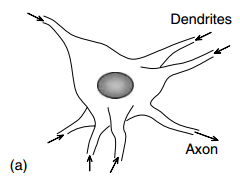
\includegraphics[width=0.8\linewidth]{./figures/neuron.PNG}
    \caption{Biological Neuron\label{fig:neuron}}
    \endminipage
    \minipage{0.5\textwidth}
    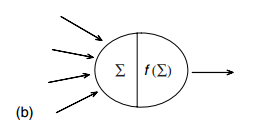
\includegraphics[width=0.8\linewidth]{./figures/math_neuron.PNG}
    \caption{Neural Model\label{fig:math_neuron}}
    \endminipage
  \end{figure}

  Haykin\cite{Haykin:1998:NNC:521706} states that “A neural network is
  a massively parallel distributed processor that has a natural
  propensity for storing experiential knowledge and making it
  available for use. It resembles the brain in two respects: 1.
  Knowledge is acquired by the network through a learning process; 2.
  Interconnection strengths between neurons, known as synaptic weights
  or weights, are used to store knowledge.” See
  \cref{fig:neural_network}.

  \begin{figure}[h]
    \begin{center}
      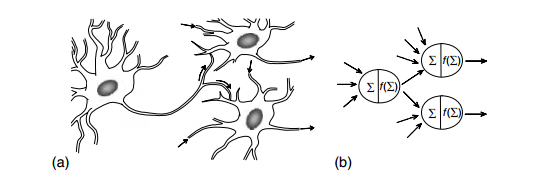
\includegraphics[width=0.8\textwidth]{./figures/neural_networks.PNG}
      \caption{Communication between neurons: (a) network of three biological
neurons, (b) neural network model.\label{fig:neural_network}}
    \end{center}
  \end{figure}

  Therefore, to mimic biological neural, scientists need to figure
  out:
  \begin{enumerate}
    \item How neurons are interconnected.
    \item How to get the weight of connections and update them by
      learning.
    \item How signal is processed locally in one neuron.
  \end{enumerate}

  To summarize, a neural network is a collection of interconnected
  neurons that incrementally learn from their environment (data) to
  capture essential linear and nonlinear trends in complex data, so
  that it provides reliable predictions for new situations containing
  even noisy and partial information.  Neurons are the basic computing
  units that perform local data processing inside a network. These
  neurons form massively parallel networks, whose function is
  determined by the network structure (i.e., how neurons are organized
  and linked to each other), the connection strengths between neurons,
  and the processing performed at neurons.

  The problem with this definition is that neuroscientist does not know
  how exactly information is processed in one neuron, which provides
  researchers with an opportunity to experiment with new ideas for these
  networks, resulting in a rich array of neural networks. Those neural
  networks in nature are linear or nonlinear fitting of one arbitrary
  function. So it is still mathematics in another form.  By using
  nonlinear function in each mathematical neuron, for instance, sigmoid
  function, the combination of those neurons could fitting any nonlinear
  function given enough number of neurons -- one neuron could fit one
  time's change of montonicity.

  It may be possible that human brain is just fitting a rather complex
  nonlinear function, however, the computational complexity limits the
  number of layers to only to normally three, called shallow neural
  network, which significantly limits the power of aritifical neural
  network.

  \section{Deep Neural Network}

  The limitation of neural network makes it unpopular until the
  resurrection of deep neural network only recently. A large amount of
  efforts are focused on learning intermediate representation of input
  samples instead of learning the fitting function directly. This
  approach proves to be of great success.

  Humans are exposed to myriad of sensory data received every second
  of the day and are somehow able to capture critical aspects of this
  data in a way that allows for its future use in a concise manner.
  Over 50 years ago, Richard Bellman, who introduced dynamic
  programming theory and pioneered the field of optimal control,
  asserted that high dimensionality of data is a fundamental hurdle in
  many science and engineering applications. The main difficulty that
  arises, particularly in the context of pattern classification
  applications, is that the learning complexity grows exponentially
  with linear increase in the dimensionality of the
  data\cite{Arel:2010:RFD:1921914.1921920}.

  Recent neuroscience findings have provided insight into the
  principles governing information representation in the mammalian
  brain, leading to new ideas for designing systems that represent
  information.  One of the key findings has been that the neocortex,
  which is associated with many cognitive abilities, does not
  explicitly pre-process sensory signals, but rather allows them to
  propagate through a complex hierarchy of modules that, over
  time, learn to represent observations based on the regularities they
  exhibit. This discovery motivated the emergence of the subfield of
  deep machine learning, which focuses on computational models for
  information representation that exhibit similar characteristics to
  that of the neocortex\cite{Arel:2010:RFD:1921914.1921920}.

  In addition to the spatial dimensionality of real-life data, the
  temporal component also plays a key role. An observed sequence of
  patterns often conveys a meaning to the observer, whereby
  independent fragments of this sequence would be hard to decipher in
  isolation.  Meaning is often inferred from events or observations
  that are received closely in time. To that end, modeling the
  temporal component of the observations plays a critical role in
  effective information representation. Capturing spatiotemporal
  dependencies, based on regularities in the observations, is
  therefore viewed as a fundamental goal for deep learning systems\cite{Arel:2010:RFD:1921914.1921920}.

  Assuming robust deep learning is achieved, it would be possible to
  train such a hierarchical network on a large set of observations and
  later extract signals from this network to a relatively simple
  classification engine for the purpose of robust pattern recognition.
  Robustness here refers to the ability to exhibit classification
  invariance to a diverse range of transformations and distortions,
  including noise, scale, rotation, various lighting conditions,
  displacement, etc\cite{Arel:2010:RFD:1921914.1921920}.

  In 2012, Google researchers collaborating with Stanford Associate
  Professor Andrew Ng, announced a breakthrough on a project dubbed
  “Google Brain.” They built software that analyzed 10 million photos
  taken from YouTube videos and learned to recognize thousands of
  objects, including human and cat faces, without human guidance. Since
  then, U.S.  tech giants have competed to hire leading figures in the
  relatively small field\cite{deep_learning_mit_tech_review}. In NLP field, deep learing demonstrates its
  capability by a technique called word embedding. In
  \cite{DBLP:journals/corr/abs-1103-0398}, the author uses Deep Neural
  Network to get a real-value feature vector of each word, which proves
  to capture linguistic regularities and patterns, and empowered with
  the new learned, the new NLP approach achieves or exceeds
  state-of-the-art performance in part-of-speech tagging, chunking,
  named entity recognition and semantic role labeling tasks.

  However, despite the success in a number of fields, such as Computer
  Vision, Natural Language Processing, why such a representation is
  able to capture the linguistic features underlying one word and its
  embedding context is still unclear. Just as the dicussion of
  mechanism of neural nework in previous section, neural network is
  mathematically equivalent to fitting data into one nonlinear
  function, which gives no intuitive interpretation.

  Understanding natural language is a tough task, so is giving an
  explanation of why word embedding works. We get started by verifying
  simple assumptions. In this context, since the main strength of neural
  network is its capability to capture nonlinear information in
  whatsoever probabilistic space of natural language, we may ask is the
  ability to recognize all kinds of nonlinear features of natural
  language that makes it stands out? This brings forward the question:
  how could we measure nonlinearity?

  Inspired by the theoretical sound probabilistic model in natural
  language -- \textbf{Topic Model}, we tackle this problem in a
  probabilistic view. The introduction of topic model will be held for
  the time being.  Nonlinearity relation between variables means the
  existence of higher order statistic. Therefore, we are going to try
  figuring out whether higher order statistic matters in NL. This idea
  is also motivated by the already made discussion in Computational
  Vision(CV) field. By learning how the comparison is made between
  methods only utilizing second order statistic and the one that
  utilizes higher order statistic in CV, we try to do research on the
  statistic of NL.

  \section{Computional Vision}
  \textit{NOTE: This section wholely references \cite{Hyvrinen09}.}

    \subsection{Background}


    The first step to solve a problem is to formalize the problem. The
    effectiveness of the formalization in some sense determine whether the
    problem is solvable or not. In CV, the first step is to define
    \textbf{what is vison}?

    We can define vision as the process of acquiring knowledge about
    environmental objects and events by extracting information from the
    light the object emit or reflect. The first thing we will need to
    consider is in what form this information initially is available.

    The light emitted and reflected by objects has to be collected and
    then measured before any information can be extracted from it. Both
    biological and artificial systems typically perform the first step by
    projecting light to form a two-dimensional image. From the image, the
    intensity of the light is then measured in a large number of spatial
    locations or sampled.

    More formally, an image $I$ is formalized as following:

    \begin{definition}
      \textbf{Image}: An image $I$ is a tuple of $(f, P)$, where $P$ is
      the set of spatial points $(x, y)$ contained in this image and $f$
      is a scalar function map spatial points $(x, y)$ to a value
      belongs to some arbitrary set, for instance, most image used in CV
      is 64 level grey scale value, which means a set of integer in $\{
      1, \ldots, 64\}$.
    \end{definition}

    For convenience, we denote the mapping $f(x, y)$ as $I(x, y)$.

    \begin{figure}[h]
      \begin{center}
        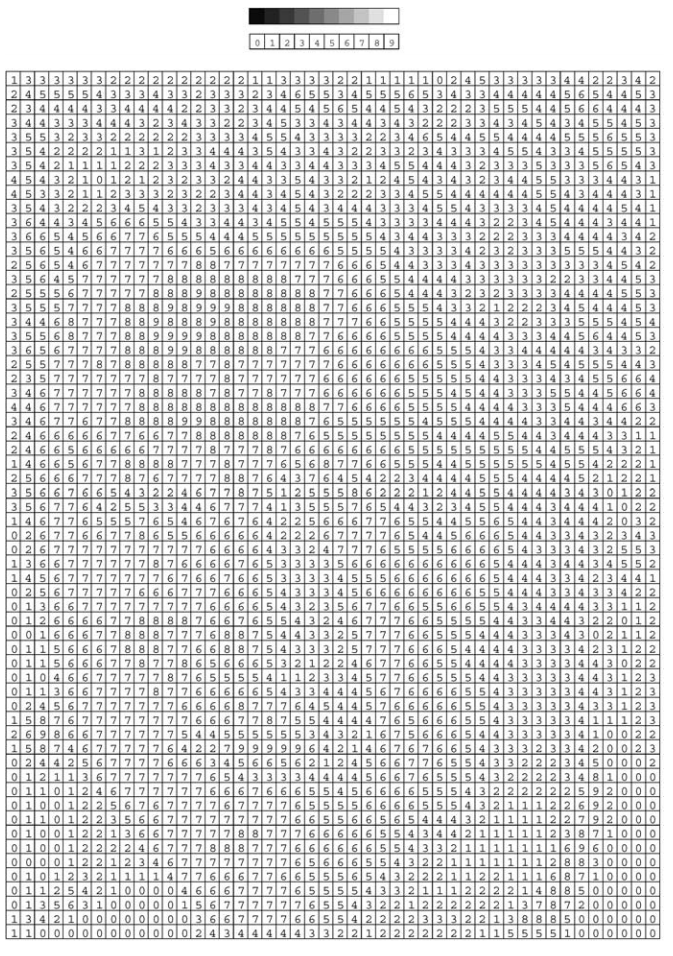
\includegraphics[width=0.8\textwidth]{./figures/numerical_image.PNG}
        \caption{An image displayed in numerical format. The shade of
          grey of each square has been replaced by the corresponding
          numerical intensity value. What does this mystery image
          depict\label{fig:numerical_image}}
      \end{center}
    \end{figure}

    \begin{figure}[h]
      \begin{center}
        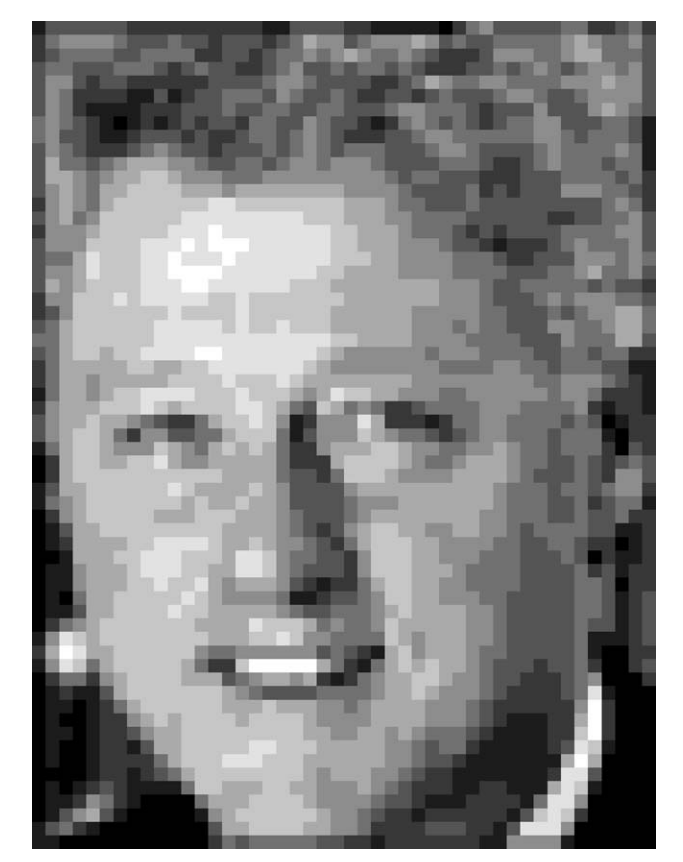
\includegraphics[width=0.8\textwidth]{./figures/image_demo.PNG}
        \caption{The image of \cref{fig:numerical_image}. It is
          immediately clear that the image shows a male face. Many
          observers will probably even recognize the specific individual
          (note that it might help to view the image from relatively far
          away)\label{fig:image_demo}}
      \end{center}
    \end{figure}

    It is from this kind of image data that vision extracts information.
    Information about the physical environment is contained in such
    images, but only implicitly. The visual system must somehow transform
    this implicit information into an explicit form, for example by
    recognizing the identities of objects in the environment. The visual
    system must convert \cref{fig:numerical_image} into the face
    \cref{fig:image_demo} we can recognize.

    This is a hard problem. However, this brings forward the importance of
    learning intermediate representation based on adaptation to the
    statistics of the input. An adaptative representation is one that does
    not attempt to represent all possible kinds of data; instead, the
    representation is adapted to represent a particular kind of data. Thus
    the visual system is not viewed as a general signal processing machine
    or a general problem-solving system. Instead, it is acknowledged that
    it has evolved to solve some very particular problems that form a
    small subset of all possible problems.

    \subsection{Generative Model}

    In vision research, more and more emphasis is being laid on the
    importance of the enormous amount of prior information that the
    brain has about the structure of the world. A formalization of these
    concepts has recently been pursued under the heading ``Bayesian
    perception'', although the principle goes back to the ``maximum
    likelihood principle'' by Helmholtz in the 19th century. Bayesian
    inference is the natural theory to use when inexact and incomplete
    information is combined with prior information. Such prior
    information should presumably be reflected in the whole visual
    system.

    It conforms with the prosperity of bayesian statistics in 20th
    century, which is also a great application to understand bayes.
    Bayesian statistics is a subset of the field of statistics in which
    the evidence about the true state of the world is expressed in terms
    of degrees of belief or, more specifically, Bayesian
    probabilities\cite{wiki_bayesian_probability}, which is introduced
    in section \ref{sec:bayesian_probability}.

    Bayesian inference formalizes how to use prior information in the
    visual system. More formally, bayesian inference refers to
    statistically estimating the hidden variables $s$ given an observed
    image $I$, where $s$ is a vector of hidden variables. The hidden
    variables are considered to contain essential structure that are
    relevant to our visual system. In most model, it is impossible (even
    in theory) to know the precise values of $s$, so it is natural to
    only to estimate a probabilistic model.

    More formally, to find out the underlying variables that determine
    or influence visual system, we estimate probability density
    $p(s|I)$, which connects to bayes -- given the observed image $I$ to
    calculate latent variables $s$. Using Bayes' rule, we can
    reformulate the probability density:

    \begin{displaymath}
      p(s|I) = \frac{p(I|s)p(s)}{p(I)}
    \end{displaymath}

    The problem becomes estimate $p(I|s)$ given a prior $p(s)$. In
    Bayesian inference, prior information is subjective, which means we
    choose which kind of probability density the latent variables will
    performs. Different priors will result in different probability
    density of $p(s|I)$ and different computational complexity.

    The idea connects back to the discussion of our biological adapted
    visual system. $p(s)$ is the mathematical abstraction of the
    ecological adapted prior information in your visual system. We are
    seeing a particular kinds of information generated by hidden
    structure(variables) $s$, which means $p(I|s)$. This approach in
    statistics or ML is called \textbf{Generative Model}. 

    And $s$ connects to the idea of intermediate representation we are
    discussing throughout this thesis.

    \subsection{Prior With Different Statistic Order in CV}
    As emphasized when introducing Bayesian Probability, the idea of
    bayes is to combine objective oberservation and subjective belief. We
    decide what kind of structure the hidden variable $s$ will have.
    This brings out different prior distribution we could assume for
    visual system. Our assumption or hypothesis determines the output we
    may get. Computional Vision researcher has put a great amount
    of effort in understanding the characteristics of the distribution
    of variable $s$.

    One major milestone in CV is to recognize the $s$ is nongaussian,
    which means it contains higher order statistic information. An
    intuitive illustration is to think about natural image in nature.
    Objects mainly consist of surfaces which are relatively uniform in
    color, meaning it has little fluctuation. There are peaks around the
    edges of surfaces. After removing the DC component of one image, we
    could expect that in most area of the image, it is around zero,
    while some peaks in some area. This brings about the idea of
    \textbf{sparseness} in CV. More formally, sparseness means that the
    random variable is most of the time very close to zero and only
    occasionally gets clearly non-zero values. One often says that
    random variable is ``active'' only rarely.

    To model sparseness mathematically, idea of using higher order
    moment is brought out, for instance, kurtosis, which is the fourth
    moment in statistics.  Therefore, $s$ is expected not to be only
    gaussian, which only utilizes second order statistic, meaning
    covariance in the data. And the hypothesis is verified by
    Computational Vision Reseachers.

    \begin{remark}
      The DC component refers to the mean grey-scale value of the pixels
      in an image or an image patch.
    \end{remark}

    This brings about what I would like to do on Natural Language. In
    next chapter, I will discuss the technique used by CV reseachers to
    verify this hypothesis and apply them on natural language later.


\chapter{Methods Exploring Different Order Statistic}
\label{chp:exploring_different_stat}

Before moving on, the developing thread of this thesis should be
stressed. In chapter \ref{chp:linear_algebra} and chapter
\ref{chp:matrix_calculus}, relavant linear algebra and matrix calculus
knowledge are introduced, while in chapter \ref{chp:probability_theory},
probability theory is introduced from scratch. To the best of my
knowledge, algebra(including linear algebra, matrix algebra and etc)
gives the players(mathematical object) and playground(mathematical
space) while probability theory gives mathematical abstraction to reason
with uncertainty using the players and playground. All those mathematics
combined with advance in neuroscience cross-validate the point that it
matters to learn intermediate representation. In algebra, it is a lower
dimension set of basis that matters while in probability theory, it is
hidden random variables. Returning back to nature, human brain does one
layer of abstraction following another to formulate concepts.

Since the variables are hidden, we can only find out its characteristics by
observing and verifying assumptions. In this chapter, I will describe
two methods, Factor Analysis and Independent Component Analysis, to
explore the statistical characteristics of data. Factor Analysis only
utilizes second order statistic while Independent Component Analysis is
the technique created to capture higher order statistic information.
Before that, I will give some explanation on the intuition behind
multivariate statistics.

  \section{Multivariate Statistics}

  We have emphasized the idea that matrix is a tool mathematicians
  created to combat complexity of the world and it is viewed as an array
  of numbers or a representation of linear transformation. Multivariate
  Statistics is an great example to illustrate the former point. A large
  data set is bulky, and its very mass poses a serious obstacle to any
  attempt to visually extract pertinent information. Much of the
  information contained in the data can be assessed by calculating
  certain summary numbers, known as \textbf{descriptive
    statistics}\cite{johnson2007applied}. Correlation coefficient is an
  example.

    \subsection{Intuition of Correlation Coefficient}

    First we introduce the idea in univariate form.

    \begin{definition}
      If $X$ and $Y$ are jointly distributed random variables with
      expectations $\mu_X$ and $\mu_Y$, respectively, the Correlation
      Coefficient of $X$ and $Y$ is:
      \begin{displaymath}
        \rho_{X,Y} = coor(X,Y) = \frac{cov(X,Y)}{\sigma_X\sigma_Y} = \frac{E[(X
        - \mu_X)(Y - \mu_Y)]}{\sigma_X\sigma_Y}
      \end{displaymath}
    \end{definition}

    The intuition behind it is linear coorelation: If the random variables
    are positively associated—that is, when X is larger than its mean, Y
    tends to be larger than its mean as well—the covariance will be
    positive. If the association is negative—that is, when X is larger
    than its mean, Y tends to be smaller than its mean -- the covariance
    is negative.\cite{rice2007mathematical}

    Actually, this is called \textit{Pearson's product-moment
    coefficient}.\cite{wiki_Correlation_and_dependence} There are other ways or intuition to analyze the
    relationship between variables, such as mutual information.

    \subsection{Correlation Matrix}

    What if we are given more than two random variables, which is the
    case in real world? A measure of linear association between the
    measurements of multiple variables is in the form of covariance
    matrix(covariance is unnormalized correlation coefficient). More
    formally, given a random vector $x \in R^{m}$(for notation
    simplicity, we assume its mean is zero), sampled $n$ times, its
    sample covariance is defined as
    $\frac{1}{n}\sum\limits^{n}_{i=1}xx^{T}$, denoted $\Sigma$, which
    has been used at the beginning of this thesis in Spetral
    Decomposition. To make it make more sense, $\Sigma_{ij} =
    \frac{1}{n}\sum\limits^{n}_{k=1}x_{i}x_{j}$. If mean of $x$ is not
    zero, the formula will become the more familiar one:
    $\frac{1}{n}\sum\limits^{n}_{k=1}(x_{i} - \bar{x_{i}})(x_{j} -
      \bar{x_{j}})$, which is the univariate case introduced previous
      section.

    \subsection{PCA Revisit Again}
    Remember that at the time we are trying to solve the problem PCA
    poses, the only thing we do is actually finding the eigenvector of
    covariance matrix of the dataset. Covariance matrix is one technique
    of descriptive statistic, which only captures second order statistic
    information. And PCA's capability stops at second order statistic.
    This will be more clear when we finish discussing factor analysis.

  \section{Factor Analysis}
  Before going higher order statistic, we introduce the generalized form
  of PCA, which is called \textbf{Factor Analysis}. This section wholely
  references \cite{johnson2007applied}.

  We start with an example.

  \begin{example}
    (\textbf{Factor Analysis of consumer-preference data})

    In a consumer-preference study, a random sample of customers were asked to
    rate several attributes of a new product. The responses, on a 7-point
    semantic differential scale, were tabulated and the attribute correlation
    matrix constructed. The correlation matrix is prsented next:

    \begin{table}[h]
      \centering
      \begin{tabular}{cccccc}
        \toprule[1.5pt]
        \head{Attribute/Variable}   & \head{1}  & \head{2}  & \head{3}  & \head{4}  & \head{5} \\
        \midrule
        Taste                       & 1.00      & 0.02      & 0.96      &    0.42   & 0.01 \\
        Good buy for money          & 0.02      & 1.00      & 0.13      &    0.71   & 0.85 \\
        Flavor                      & 0.96      & 0.13      & 1.00      &    0.50   & 0.11 \\
        Suitable for snack          & 0.42      & 0.71      & 0.50      &    1.00   & 0.79 \\
        Provides lots of energy     & 0.01      & 0.85      & 0.11      &    0.79   & 1.00 \\
        \bottomrule[1.5pt]
      \end{tabular}
      \caption{consumer-preference data\label{tab:consumer_preference_data}}
    \end{table}

    Rewrite coorelation data in matrix form, we have:

    \begin{displaymath}
      \begin{bmatrix}
         1.00      & 0.02      & \underline{0.96}      &    0.42   & 0.01 \\
         0.02      & 1.00      & 0.13      &    0.71   & \underline{0.85} \\
         0.96      & 0.13      & 1.00      &    0.50   & 0.11 \\
         0.42      & 0.71      & 0.50      &    1.00   & \underline{0.79} \\
         0.01      & 0.85      & 0.11      &    0.79   & 1.00
      \end{bmatrix}
    \end{displaymath}

    From the underlined correlation number, we can infer that variable 1 and 3
    form group while variable 2 and 5 form one group. Variable 4 is ``closer''
    to the (2, 5) group. Given these results and the small number of variables
    we might expect that the apparent \textbf{linear relationships} between the
    variables be explained in terms of, at most, two or three common factors.
  \end{example}

  How could we find out those hidden factors? To reason with uncertainty, we
  need to make assumption. In the context of intermediate representation or
  bayesian inference, they are called prior  knowledge or subjective belief. In
  the following content, formal factor analysis model will be introduced.

  Given the observable random vector $X$, with $p$ components, has mean
  $\mu$ and covariance matrix $\Sigma$, the factor model postulates that $X$ is
  linearly dependent upon a few unobservable random variables $F_{1}, F_{2},
  ... , F_{m}$, called common factors, and $p$ additional sources of variation
  $\epsilon_{1}, \epsilon{2}, ... , \epsilon{p}$, called errors or sometimes,
  \textit{specific factors}. In particular, the factor analysis model is

  \begin{align*}
    X_{1} - \mu_{1} &= l_{11}F_{1} + l_{12}F_{2} + \cdots + l_{1m}F_{m} + \epsilon_{1}\\
    X_{2} - \mu_{2} &= l_{21}F_{1} + l_{22}F_{2} + \cdots + l_{2m}F_{m} + \epsilon_{2}\\
    \vdots          &= \vdots \\
    X_{p} - \mu_{p} &= l_{p1}F_{1} + l_{p2}F_{2} + \cdots + l_{pm}F_{m} + \epsilon_{p}\\
  \end{align*}

  Rewrite it in matrix formula, we have:

  \begin{displaymath}
    \underset{p \times 1}{X - \mu} = \underset{p \times m}{L}\underset{m \times
      1}{F} + \underset{p \times 1}\epsilon
  \end{displaymath}

  The coefficient $l_{ij}$ is called the loading of the $i$th variable on the
  $j$th factor, so the matrix $L$ is the \textit{matrix of facts loading}. With
  so many unobservable quantities, a direct verification of the factor model
  from observations on $X_{1}, X_{2}, ... , X_{p}$ is hopeless. However, with
  some additional assumptions about the randome vectors $F$ and $\epsilon$, the
  model implies certain covariance relationships, which can be checked.

  We assume that
  \begin{displaymath}
    E(F) = \underset{m \times 1}{0} 
  \end{displaymath}

  \begin{displaymath}
    Cov(F) = E(FF') = \underset{m \times m}{I}
  \end{displaymath}

  \begin{displaymath}
    E(\epsilon) = \underset{p \times 1}{0}
  \end{displaymath}

  \begin{displaymath}
    Cov(\epsilon) = E(\epsilon \epsilon') = \Psi = 
    \begin{bmatrix}
      \Psi_{1}  & 0             & \cdots & 0 \\
      0             & \Psi_{2}  & \cdots & 0 \\
      \vdots        & \vdots        & \ddots & \vdots \\
      0             & 0             & \cdots & \Psi_{p} \\
    \end{bmatrix}
  \end{displaymath}

  $F$ and $\epsilon$ are independent, so

  \begin{displaymath}
    Cov(\epsilon, F) = E(\epsilon F') = \underset{p \times m}{0}
  \end{displaymath}

  With those assumptions, we return back to the covariance matrix:

  \begin{align*}
    (X - \mu)(X - \mu)' &= (LF + \epsilon)(LF + \epsilon)'                  \\
                        &= (LF + \epsilon)((LF)' + \epsilon')               \\
                        &= LF(LF)' + \epsilon(LF)' + LF\epsilon' + \epsilon
                        \epsilon'                                           
  \end{align*}

  So that,
  \begin{align*}
    \Sigma  &= Cov(X) = E(X - \mu)(X - \mu)'                              \\
            &= LE(FF')L + E(\epsilon F')L' + LE(F\epsilon') + E(\epsilon
            \epsilon')                                                    \\
            &= LL' + \Psi
  \end{align*}

  This equation brings us back to spectral decomposition in section
  \ref{sec:spectral_decomposition}. Spectral decomposition provides us with one
  factoring of the covariance matrix $\Sigma$. Let $\Sigma$ have
  eigenvalue-eigenvector $(\lambda_{i}, e_{i})$ with $\lambda_{1} \geq
  \lambda_{2} \geq \cdots \geq \lambda_{p} \geq 0$. Then

  \begin{align*}
    \Sigma  &= \lambda_{1}e_{1}e_{1}' + \lambda_{2}e_{2}e_{2}' + \cdots +
      \lambda_{p}e_{p}e_{p}' \\
            &= 
            \begin{bmatrix}
              \sqrt{\lambda_{1}}e_{1} & \sqrt{\lambda_{2}}e_{2} & \cdots & \sqrt{\lambda_{p}}e_{p}
            \end{bmatrix}
            \begin{bmatrix}
              \sqrt{\lambda_{1}}e_{1} \\
              \sqrt{\lambda_{2}}e_{2} \\
              \vdots \\
              \sqrt{\lambda_{p}}e_{p}
            \end{bmatrix}
  \end{align*}

  This fits the prescribed covariance structure for the factor analysis model
  having as many factors as variables ($m = p$) and specific variances $\psi_{i}
  = 0$ for all $i$. The loading matrix has $j$th column given by $
  \sqrt{\lambda_{j}}e_{j}$. That is, we can write
    \begin{displaymath}
      \underset{p \times p}{\Sigma} = \underset{p \times p}{LL'} + \underset{p
        \times p}{0} = LL'
    \end{displaymath}

    Just as the case of trucated SVD, we cut off eigenvalues that diminishes.
    Then we can get the loading matrix. This must bring you the connection with
    PCA. Actually, PCA is a special case of Factor Analysis(FA). The difference
    between PCA and FA is that PCA does not have any error assumption $\Psi$
    while FA takes into account error. The error term $\Psi$ is usually assumed
    to be gaussian since the derivation of factor matrix only takes advantages
    of covariance matrix, which only takes into account second order statistic,
    and gaussian distribution can be determined from one order and second order
    statistic. After an assumption about the error term $\Psi$, we can get
    factor matrix $F$ just by solving regular linear equations.

  \section{Second Order Statistic Is Not Enough}

  The intuition behind is already explained in the context of CV in
  previous chapter. The difference in assumption of prior distribution
  already makes a great difference. In this section, I will gives more
  mathematical intrepretation about the intuition, to illustrate that
  information is being ignored by just using gaussian assumption.

  Gaussian Distribution gains its reputation mainly because its
  simplicity, but it is also its simplicity that makes it less capable.
  First, gaussian distribution is spherically symmetric; Second, as long
  as two gaussian distributions are linear uncorrelated, they are
  independent. For real world data distributions, it is obvious that
  they do not hold. In the following of this section, I will introduce
  orthogonal transformation and point out that under orthogonal
  transformation, gaussian distributions are unidentifiable, in another
  word, with gaussian assumption, the best we can get is recovering
  second order statistic information.

    \subsection{Orthogonal Transformation}
    \label{sec:orthogonal_transformation}
    At the time we introduce matrix, we say that there are two ways to
    view matrix, a rectangular array of numbers and an compact
    representation of linear transformation. We have gives an example of
    former view when introducing factor analysis. Here we introduce
    another view of matrix.

    First we define related definitions.

    \begin{definition}
      \textbf{Orthogonal Matrix}: given one matrix $Q$, if $QQ^{T} = I$,
      then $Q$ is called orthogonal matrix.
    \end{definition}

    \begin{definition}
      \textbf{Orthogonal Transformation}: given an orthogonal matrix $Q$,
      then for any vector $x$, $Qx$ is called an orthogonal transformation
      of $x$.
    \end{definition}

    Orthogonal transformation has the following properties:
    \begin{enumerate}
      \item Orthogonal transformation preserves length of original vectors.
      \item Orthogonal transformation preserves angle of original vectors.
    \end{enumerate}

    Proof is omitted. And they are not hard.

    To make it make more sense, orthogonal transformations in two- or
    three-dimensional Euclidean space are stiff rotations, reflections, or
    combinations of a rotation and a
    reflection\cite{wiki_orthogonal_transformation}.

    Since orthogonal transformation preserves length and angle, it could
    be viewed as a change of basis in the vector space, which could be
    viewed as another property of orthogonal transformation -- orthogonal
    transformation map orthonormal bases to orthonormal bases. This also
    could be connect back to eigenvalue and spectral decomposition
    introduced previously. Remember that given any real symmetric matrix
    $A$, it can be decomposed into the form $Q\Sigma Q^{T}$, where columns
    of $Q$ are orthonormal eigenvectors of $A$ and diagonal of $\Sigma$
    are eigenvalues of $A$. It means that matrices with the same set of
    eigenvalues are just different representations in different basis and
    eigenvalues are the key to connect them.

    \subsection{Whitened Gaussian pdf is Spherically Symmetric}

    We illustrate this in algebra and probabilistic perspectives.

      \subsubsection{Algebra Perspective}
      We use PCA to illustrate. If you forget the notation, return back
      to chapter \ref{chp:matrix_calculus} to refresh yourselves. Given
      dataset $X$, we obtain lower dimensional intermediate
      representation by computing its covariance matrix $\Sigma$'s eigenvectors
      $Z$. Then $X = WZ^{T}$, where $W$ is the score we want. However, given
      any orthonormal matrix $Q$, if we replace $Z$ with $QZ$.
      Correspondingly, $\Sigma = Z\Lambda Z^{T}$ becomes $Q\Sigma Q^{T}
      = QZ\Lambda Z^{T}Q^{T}$ and $X = WQQ^{T}Z^{T} = WZ^{T}$.

      We still get $X$, but $W$, actually $WQ$, is not the same anymore,
      which means PCA, a.k.a gaussian distribution cannot identify
      orthonormal transformation. PCA can recover the best linear
      subspace in which the signals lie, but cannot uniquely recover the
      signals themselves.

      \subsubsection{Probabilistic Perspective}
      This view clearly explains where is the limit of the information
      PCA can reach. In the ICA to be introduced next, PCA is one part
      of it, which does the job to center and whiten the data. Centering
      is another way of calling removing DC component in CV. It computes
      the mean of each dimension of the data and removes it from them,
      thus centering each dimension at zero. Whitening is to tranform
      the covariance matrix into identity matrix(meaning they are
      uncorrelated and all have variance 1). By such preprocessing, no
      information can be provided by first and second order statistic.
      This is what ``the best PCA can get is recovering second order
      statistic information'' means.  Those two are regarded as
      preprocessing of data before the core procedure of ICA begins. But
      note that ICA may discard some dimensions that are of too small
      eigenvalues to reduce the computation complexity.

      After whitening, spherically symmetric directly reflects on the
      gaussian distribution. The whitened multivariate gaussian pdf
      shows as following:

      \begin{displaymath}
        p(x_{1}, \ldots, x_{n}) =
        \frac{1}{(2\pi)^{\frac{n}{2}}}exp(-\frac{1}{2}\sum\limits^{}_{i}x_{i}^{2})
        = \frac{1}{(2\pi)^{\frac{n}{2}}}exp(-\frac{1}{2}||x||^{2})
      \end{displaymath}

      The pdf only depends on the norm of $x$, so it is spherically
      symmetric.

      \subsection{Uncorrelated Gaussian Variables Are Independent} Using
      gaussian assumption, we are not take advantage of independence
      assumption made about the hidden variables\cite{Hyvrinen09}. For
      random variables $s_{1}, \ldots, s_{n}$ have a gaussian
      distribution and they are uncorrelated, then they are also
      independent. Thus, for gaussian variables, uncorrelatedness and
      independence are the same thing, although in general they are not.
      This is also another point of view that PCA can only decorrelate
      data but not extracting further information.

      Mathematically, it is easy to see that $p(x_{1}, \ldots, x_{n})$
      can be factorized:

      \begin{displaymath}
        p(x_{1}, \ldots, x_{n}) =
        \prod\limits_{i}\frac{1}{\sqrt{2\pi}}exp(-\frac{1}{2}x_{i}^{2})
      \end{displaymath}

      which means they are independent.

  \section{Independent Component Analysis}
  So how could we make use of higher order statistic information
  contained in data? Beyond linearity, there are a number of nonlinear
  characteristics may be captured. Remember that it is the intuition of
  not capturing sparseness information in natural image that makes us
  think about taking advantage of higher order statistic. Thus
  researchers actually begins by maximize sparseness contained in
  natural image\cite{Hyvrinen09}. Then the intuition is generalized to
  maximize non-gaussian characteristics.  Super-Gaussianity is basically
  the same as sparseness and there are information in natural image that
  are beyond sparseness\cite{Hyvrinen09}. Super-Gaussianity will be
  introduced later.

  Therefore, to capture non-gaussianity in natural image,
  \textbf{Independent Component Analysis} shows its appearance.

    \subsection{Definition}
    To rigorously define ICA, we can use a statistical ``latent
    variables'' model\cite{hyvärinen2004independent}. We observe $n$
    random random variables $x_{1}, \ldots, x_{n}$, which are modeled as
    linear combination of $n$ random variables $s_{1}, \ldots, s_{n}$:
    \begin{displaymath}
      x_{i} = a_{i1}s_{1} + a_{i2}s_{2} + \ldots + a_{in}s_{n},
      \text{for all $i = 1, \ldots, n$}
    \end{displaymath}

    Rewrite it in the form of matrix:

    \begin{equation}
      x = As
      \label{eq:ica}
    \end{equation}

    This is the basic ICA model. In more complex model, the dimension of
    $x$ could be different from $s$, time series is not taken into
    consideration and noise could be added. The intuition behind this
    model is to generate observed data from mixing non-gaussian hidden
    variables $s$, thus it is a generative model.  More specifically,
    the independent components $s$ are latent variables which could not
    be observed directly. Also, the mixing coefficients $a_{ij}$ are
    assumed to be unknown. All we observe are the random variables
    $x_{i}$ and we must estimate both the mixing coefficients $a_{ij}$
    and $s$ using $x$. This must be done under as general assumptions as
    possible.

    \subsection{Assumption of ICA}

      \subsubsection{Independence}

      \paragraph{The independent components are assumed statistically
        independent}.

      This is the principle on which ICA rests. Surprisingly, not much
      more than this assumption is needed to ascertain that the model
      can be estimated. This is why ICA is such a powerful method with
      applications in many different areas.

      \subsubsection{Nongaussian}

      \paragraph{The independent components must have nongaussian
        distributions}.

      In the preprocessing step of ICA, all information in first and
      second statistic of the data are used up. ICA aims at discovering
      information that hidden in higher order statistic. Thus, ICA is
      essentially impossible if the observed variables have gaussian
      distributions. Note that in the basic model, we do \textit{not}
      assume that we know waht the nongaussian distributions of $s$ look
      like; if they are known, the problem will be considerably
      simplified.

      \subsubsection{Square}

      \paragraph{For illustration of the intuition behind, we assume
        that the unknown mixing matrix is square}.

      In other words, which is mentioned before, the number of
      independent components is equal to the number of observed
      mixtures. This assumption can be relatexed. For detail, please see
      \cite{hyvärinen2004independent}.

    \subsection{Ambiguities of ICA}

    In equation \ref{eq:ica}, it is easy to see that the following
    ambiguities or indeterminacies will necessarily hold:

    1. we cannot determine the variances of the independent components.

    The reason is that, both $s$ and $A$ being unknown, any scalar
    multiplier in one of the sources $s_{i}$ could always be canceled by
    dividing the corresponding column $a_i$ of $A$ by the same scalar,
    say $\alpha_{i}$:

    \begin{displaymath}
      x = \sum\limits^{}_{i}(\frac{1}{\alpha_{i}}a_{i})(s_{i}\alpha_{i})
    \end{displaymath}

    As a consequence, we may quite as well fix the magnitudes of the
    independent components. Since they are random variables, the most
    natural way to do this is to assume that each has unit variances:
    $E[s_{i}^{2}] = 1$. Then the matrix $A$ will be adapted in the ICA
    solution methods to take into account this restriction. Note that
    this still leaves the ambiguity of the sign.

    2. We cannot determine the order of the independent components.

    The reason is that, again both $s$ and $A$ being unknown. Their
    order can be changed freely. Formally, a permutation matrix $P$ and
    its inverse can be substituded in the model to give $x = AP^{-1}Ps$.

    \subsection{ICA by Maximize Kurtosis}

    There are several ways to implement the idea of ICA. For the purpose
    of being intuitive, and combined the intuition described in previous
    chapter in CV, we explain ICA by maximizing kurtosis to maximize the
    non-gaussian in $s$\cite{Hyvarinen:2000:ICA:351654.351659}. Note
    that the data should be centered and whitened before reaching this
    step.

    The classical measure of nongaussianity is kurtosis or the
    fourth-order cumulant. The kurtosis of $y$ is classically defined by
    \begin{displaymath}
      kurt(y) = E[y^{4}] - 3(E[y^{2}])^{2}
    \end{displaymath}

    Actually, since we assumed that $y$ is of unit variance, the
    right-hand side simplifies to $E[y^{4}] - 3$. This shows that
    kurtosis is simply a normalized version of the fourth moment
    $E[y^{4}]$. For a gaussian $y$, the fourth moment equals
    $3(E[y^{2}])^{2}$. Thus, kurtosis is zero for gaussian random
    variable. For most (but not quite all) nongaussian random variables,
    kurtosis is nonzero. Random variables that have a negative kurtosis
    are called subgaussian and those with positive kurtosis are called
    supergaussian. Subgaussian random variables have typically a
    ``flat'' pdf, which is rather constant near zero, and very small for
    larger values of the variable. A typical example is the uniform
    distribution. Supergaussian randome variables have typically a
    ``spiky'' pdf with heavy tails, i.e., the pdf is relatively large at
    zero and at large values of the variable, while being small for
    intermediate values. A typical example is the Laplace distribution.

    \begin{figure}
      \minipage{0.6\textwidth}
      \includegraphics[width=0.8\linewidth]{./figures/uniform_distribution.png}
      \caption{Uniform Distribution\label{fig:uniform_distribution}}

      \endminipage
      \minipage{0.6\textwidth}
      \includegraphics[width=0.8\linewidth]{./figures/laplace_distribution.png}
      \caption{Laplace Distribution\label{fig:laplace_distribution}}

      \endminipage\hfill
    \end{figure}

    Typically, nongaussianity is measured by the absolute value of
    kurtosis. The square of kurtosis can also be used. These are zero
    for a guassian variable and greater than zero for most nongaussian
    random variables. There are nongaussian random variables that have
    zero kurtosis, but they can be considered as very rare.

    Kurtosis, or rather its absolute value, has been widely used as a
    measure of nongaussianity in ICA and related fields. The main reason
    is its simplicity, both computational and theoretical.
    Computationally, kurtosis can be estimated simply by using the
    fourth moment of the sample data. Theoretical analysis is simplified
    because of the following linearity property: if $x_{1}$ and $x_{2}$
    are two independent random variables, it holds
    \begin{displaymath}
      kurt(x_{1} + x_{2}) = kurt(x_{1}) + kurt(x_{2})
    \end{displaymath}

    and

    \begin{displaymath}
      kurt(\alpha x_{1}) = \alpha^{4}kurt(x_{1})
    \end{displaymath}

    where, $\alpha$ is scalar.

    To illustrate in a simple example what the optimization landscape
    for kurtosis looks like, and how independent components could be
    found by kurtosis minimization or maximization, let us look at a
    2-dimensional model $x = As$. Assume that the independent components
    $s_{1}, s_{2}$ have kurtosis values $kurt(s_{1}), kurt(s_{2})$,
    respectively, both different from zero. Remember that we assumed
    that they have unit variances. We seek for one of the independent
    components as $y = w^{T}x$.

    Let us make the transformation $z = A^{T}w$. Then we have $y =
    w^{T}x = w^{T}As = z^{T}s = z_{1}s_{1} + z_{2}s_{2}$ . Now, based on
    the additive property of kurtosis, we have $kurt(y) =
    kurt(z_{1}s_{1}) + kurt(z_{2}s_{2}) = z_{1}^{4}kurt(s_{1}) +
    z^{4}_{2}kurt(s_{2})$. On the other hand, we made the constraint that
    the variance of $y$ is equal to 1, based on the same assumption
    concerning $s_{1}, s_{2}$ . This implies a constraint on $z: E[y^{2}
    = z^{2}_{1} + z^{2}_{2} = 1]$. Geometrically, this means that vector
    $z$ is constrained to the unit circle on the 2-dimensional plane.
    The optimization problem is now: what are the maxima of the function
    $| kurt(y)| = |z^{4}_{1}kurt(s1) + z_{2}^{4}kurt(s2)|$ on the unit
    circle? For simplicity, you may consider that the kurtosis are of
    the same sign, in which case it absolute value operators can be
    omitted. The graph of this function is the ``optimization
    landscape'' for the problem.

    It is not hard to show (Delfosse and Loubaton, 1995) that the maxima are
    at the points when exactly one of the elements of vector z is zero and
    the other nonzero; because of the unit circle constraint, the nonzero
    element must be equal to $1$ or $-1$. But these points are exactly the ones
    when y equals one of the independent components $±s_{i}$, and the problem has
    been solved.

    In practice we would start from some weight vector w, compute the
    direction in which the kurtosis of $y = w^{T}x$ is growing most strongly
    (if kurtosis is positive) or decreasing most strongly (if kurtosis
    is negative) based on the available sample $X$, and use a gradient
    method or one of their extensions for finding a new vector $w$. The
    example can be generalized to arbitrary dimensions, showing that
    kurtosis can theoretically be used as an optimization criterion for
    the ICA problem.

    Above is the idea of finding nongaussian hidden components, and
    kurtosis is the most intuitive explanation of it. However, kurtosis
    has also some drawbacks in practice, when its value has to be
    estimated from a measured sample. The main problem is that kurtosis
    can be very sensitive to outliers (Huber, 1985).  Its value may
    depend on only a few observations in the tails of the distribution,
    which may be erroneous or irrelevant observations. In other words,
    kurtosis is not a robust measure of nongaussianity. An algorithm
    called fastICA is the mostly widely implementation of ICA. Details
    please refer to \cite{Hyvarinen:2000:ICA:351654.351659}.

  \section{An Example}

  \begin{figure}
    \minipage{0.6\textwidth}
    \includegraphics[width=1\linewidth]{./figures/ica_demo_uniform_data.png}
    \caption{Latent Signal\label{fig:ica_demo_uniform_data.png}}

    \endminipage
    \minipage{0.6\textwidth}
    \includegraphics[width=1\linewidth]{./figures/ica_demo_data_after_linear_mixing.png}
    \caption{Observations\label{fig:ica_demo_data_after_linear_mixing.png}}

    \endminipage\hfill
    \\
    \minipage{0.6\textwidth}
    \includegraphics[width=1\linewidth]{./figures/ica_demo_pca.png}
    \caption{PCA estimate\label{fig:ica_demo_pca.png}}

    \endminipage
    \minipage{0.6\textwidth}
    \includegraphics[width=1\linewidth]{./figures/ica_demo_ica.png}
    \caption{ICA estimate\label{fig:ica_demo_ica.png}}

    \endminipage

    \begin{center}
      Illustration of ICA and PCA applied to 100 idd samples of 2d
      source signals with a uniform distribution.
    \end{center}
  \end{figure}

  To further understand what ICA does which PCA cannot. Let us consider
  an example\cite{murphy2012machine}.

  Suppose we have two independent sources with uniform distributions, as
  shown in \cref{fig:ica_demo_uniform_data.png}. Now suppose we have the
  following mixing matrix:

  \begin{displaymath}
    W = 
    \begin{pmatrix}
      2 & 3 \\
      2 & 1
    \end{pmatrix}
  \end{displaymath}

  Then we observe the data shown in
  \cref{fig:ica_demo_data_after_linear_mixing.png}(assuming no noise).
  If we apply PCA on the linear mixing data, we get
  \cref{fig:ica_demo_pca.png}. This corresponds to a whitening of the
  data. To uniquely recover the sources, we need to perform an
  additional rotation. The trouble is, there is no information in the
  symmetric Gaussian posterior to tell us which angle to rotate by. In a
  sense, PCA solves ``half'' of the problem, since it identifies the
  linear subspace; all that ICA has to do is then do identify the
  appropriate rotation. By applying ICA, we could perfectly get the
  recovered result \cref{fig:ica_demo_ica.png}.


  \section{Summarize}

  This chapter is a mathematical solution to approach the problem that
  more information could be recovered from natural image. We start from
  PCA, the general case of it, FA and by realising that they stay in the
  comfortable zone where only lower order statistic is utilized. Then we
  introduce ICA to make use of higher order statistic, or
  nongaussianity. This is how CV researchers develops their idea to
  capture nongaussian information in natural image.

\chapter{Explore Statistic in Natural Language}
Previously, we introduce how research in Computational Vision explores
different statistic of natural image. Inspired by the result of deep
neural network, a.k.a. word embedding, and the work in CV, we guess the
idea of intermediate representation and nongaussianity matters in NLP as
well. To verify this hypothesis, experiments which applies those methods
on NL are considered promising. However, due to the large scale of the
experiments unsupervised learning needed to learn intermediate
representations, normally a dedicated distributed machine learning
infrastructure is required to verify the theoretical interpretation.
What's more, a series of experiments with different scale and on
different benchmarkings should be performed. Therefore, for the time
being, we only point out potential designs of experiments, distributed
frameworks may be used and lastly, a toy illustration of the
intermediate representations will be showed.

In this chapter, we will introduce the promising potential of
unsupervised learning, which actually is learning intermediate
representations, and its call for new distributed system to cope with
very large scale data. Then some preliminary design of experiments to verify
the hypothesis are showed, and lastly a toy example learnt by Latent Semantic
Analysis, which is the name of PCA in NL field, is demonstrated.

  \section{The Boost of Scale in Unsupervised Learning}
  In chapter \ref{chp:intermediate_representation}, we touch the idea
  of using intermediate representations to capture relavant structure
  underlying observed data. Essentially, this is what unsupervised
  learning does. Compared with supervised learning, which is called
  predictive approach, unsupervised learning is called descriptive
  approach. It tries to describe future based on ``shape'' of the past.
  To further understand the analog, we look at quote:

  \begin{quote}
    When we're learning to see, nobody's telling us what the right answers
    are — we just look. Every so often, your mother says “that's a dog”, but
    that's very little information.  You'd be lucky if you got a few bits of
    information — even one bit per second — that way. The brain's visual
    system has $10^{14}$ neural connections. And you only live for $10^9$
    seconds. So it's no use learning one bit per second. You need more like
    $10^5$ bits per second. And there's only one place you can get that much
    information: from the input itself.

    — Geoffrey Hinton, 1996 (quoted in (Gorder 2006)).
  \end{quote}

  It is from the ``shape'' of the input themselves that we learn the
  information, gradually the knowledge we want. Return to our familiar
  terminology, intermediate representation is a more formal name of
  ``shape''.

  However, just as we living creatures bave been evolving for such long
  time, the input needed to formalize reasonable output is huge. For NL,
  we need a great volume of text corpus to learn the intermediate
  representation. For instance, similar word done using PCA and
  Canonical Component Analysis(CCA)\cite{dhillon_icml12_tscca} uses 100
  thousands documents to reach the marginal effect of raising the volume
  of input data corpus, while in the work of word embedding using deep
  learning, \cite{Collobert:2008:UAN:1390156.1390177} uses seven weeks
  to train a real value word vector.

  To improve the feasibility of this approach and speed up its training
  speed, corresponding computing infrastructure calls for attention.

  \section{Dedicated System For Big Data}
  Starting from Google's Big Table\cite{Chang:2006:BDS:1267308.1267323},
  Google File System\cite{Ghemawat:2003:GFS:945445.945450} and their
  open source incarnation hadoop, large efforts have been made to deal
  with the large scale of data. A major bottleneck to applying advanced
  ML programs at industrial scales is the migration of an academic
  implementation, often specialized for a small, well-controlled
  computer platform such as desktop PCs and small lab-clusters, to a
  big, less predicable platform such as a corporate cluster or the
  cloud\cite{2013arXiv1312.7651D}.  But due to different characteristics
  different machine learning algrithms possesses, they need different
  specifical distributed system.

  As far as I know, there are a number of distributed machine learning
  framework available. Petuum\cite{2013arXiv1312.7651D}, an
  implementation of parameter server, aims at algorithms that optimizes
  a loss function iteratively, which distributes parameters among
  servers and takes advantage of data's structure when scheduling. See
  \cref{fig:petuum_ps.jpg} to have an idea of its architecture topology.
  FA and ICA can be implemented using the matrix api provided by petuum.
  Spark\cite{Zaharia:2010:SCC:1863103.1863113} embodies the
  MapReduce/dataflow approach but is easier to program than hadoop.
  SimSQL\cite{Cai:2013:SDM:2463676.2465283} is a parallel, relational
  database that supports an SQL-based approach to run large-scale MCMC
  simulations. GraphLab\cite{Low+al:uai10graphlab} supports a
  graph-based abstraction for writing distributed machine learning
  codes. Giraph is another more general-purpose graph-based processing
  platform, which is widely known to be used extensively by facebook.

  \begin{figure}[h]
    \begin{center}
      \includegraphics[width=0.65\textwidth]{./figures/petuum-ps.jpg}
      \caption{Petuum Parameter Server Topology\label{fig:petuum_ps.jpg}}
    \end{center}
  \end{figure}

  To further advance the frontier of learning intermediate
  representation, dedicated distributed systems for machine learning
  should necessarily be taken into consideration.

  \section{Problem Formalization: Bag of Words Model}
  Previously, we have talked about why large scale training for
  unsupervised learning is needed and what distributed frameworks are
  avaiable. From now on, we try to design experiements to verify our
  hypothesis that capturing higher order statistic in NL is relevant.

  There are a number of models researchers are using to model natural
  language. Among them, we choose the bag of words model to explore its
  statistic information. Bag of words model is the simplest model we can
  use to capture the information contained in documents, paragraphs or
  sentences. 

  \subsection{Model Description}

  The model we use will be formally described in the following.

  Given a collection of documents $D$, first we learn a vocabulary
  dictionary based on term frequency($TF$) and document frequency($DF$).
  Words are contained almost in all documents, which means high $DF$, are
  considered stop word. Words rarely appear, which means low $TF$, are
  considered erroneous. Words other than those two are kept as words in
  the vocabulary dictionary.

  Assume that there are $n$ words in the dictionary, and $m$ documents
  in all in the collection, then first we obtain an occurrence matrix
  $C \in N^{m \times n}$, where $N$ is the set of natural number.
  $c_{ij}$ means the $jth$ word in the dictionary has occurred $c_{ij}$
  times in the $ith$ document. Then we use $tf-idf$ vectors of each
  document to replace each row of matrix $C$, and normalize each row
  using $l_{2}$ norm. We denote this new matrix $A$.

  Before we introduce what we can get from this model, we first
  describes the information it loses when using it to model natural
  language:

  \begin{itemize}
    \item It ignores the words, sentences order in natural language.
    \item It ignores the time information in the appearance of the
      documents.
    \item It does not capture the syntactic information in sentences.
    \item In this context, it ignores all structures since the matrix is
      build on the granulity of document.
  \end{itemize}

  But one task it can perform well is to determine the topic of this
  document. Imagine how we human decide what topic one document belongs
  to? We can make judgement without relying too much on the article
  structure, sytactic structure in the sentences or the order of words.
  We can tag articles solely based on the appearance of specific key
  words. Therefore, bag of words model is fine enough to extract topic
  information of documents.

  Before we move on, we introduce the idea of document space. Consider
  we have a vocabulary of size $n$, then each document can be
  represented using a $n$ dimension vector, denoted $d$. If $ith$ word
  in the dictionary occurs $p$ times in the document, the $ith$
  dimension of $d$ is $p$. Mathematically, this document delves in a
  vector space of dimension to be $n$. We call this vector space
  document space.

  \section{Experiment Design: Find Structure in Document Space}

  Just as idea described in Computional Vision -- a spatial image
  contains hidden structure underlying pixels, we think document space
  is similar. There are already theoretically sound work done similar to
  this idea. The model well known as topic
  model\cite{Blei:2012:PTM:2133806.2133826} regards that each document
  consists of multiple topics. Different document exhibits different
  proportion of topics, which represents as a distribution over topics.
  The number of topics are specified before any data bas been generated.
  Each topic is a distribution over a fixed vocabulary.

  Inspired by topic model, we take this in an algebra approach. The
  document space described above is an extremely sparse one. We want to
  find hiddle structure in it to exhibit topic information. We assume
  that there are a fixed number of topics. Using PCA, FA, and ICA, we
  try to find hidden components in such a document space. Each
  components can be viewed as a topic and they form a new set of basis.
  Each document is a point in such a new vector space, which may be
  called topic space.

  The simplistic way to benchmark the intermediate representation is to
  do document classfication using documents representation learnt from
  original document space. This experiment should give some useful
  feedback about our hypothesis.

  \section{Illustration of Intermediate Representation}
  Though I do not run experiment on large scale data, recent
  advance\cite{Halko:2011:FSR:2078879.2078881} in computing eigens of
  matrix makes it possible to train LSA with relatively little
  resources. Thus we could give an illustration of the idea of LSA.

  \subsection{Machine Learning in Python: Sklearn}

  Before we go experimenting, we going to introduce a great open source
  python library for ML: \textbf{scikit-learn}\cite{scikit-learn}.
  scikit-learn (formerly scikits.learn) is an open source machine
  learning library for the Python programming language. It features
  various classification, regression and clustering algorithms including
  support vector machines, logistic regression, naive Bayes, random
  forests, gradient boosting, k-means and DBSCAN, and is designed to
  interoperate with the Python numerical and scientific libraries NumPy
  and SciPy\cite{wiki_scikit_learn}.

  All implementation in this thesis takes the advantage of sklearn.

  \begin{figure}[h]
    \begin{center}
      \includegraphics[width=0.65\textwidth]{./figures/scikit-learn-logo.png}
      \caption{Sklearn\label{fig:sklearn_logo}}
    \end{center}
  \end{figure}

  \subsection{Dataset}

    \subsubsection{Introduction}
    The 20 Newsgroups data set is a collection of approximately 20,000
    newsgroup documents, partitioned (nearly) evenly across 20 different
    newsgroups. It was originally collected by Ken Lang, probably for
    his Newsweeder: Learning to filter netnews paper, though he does not
    explicitly mention this collection. The 20 newsgroups collection has
    become a popular data set for experiments in text applications of
    machine learning techniques, such as text classification and text
    clustering\cite{20newsgroups}.

    \subsubsection{Organization}
    The data is organized into 20 different newsgroups, each corresponding
    to a different topic. Some of the newsgroups are very closely related to
    each other (e.g. comp.sys.ibm.pc.hardware / comp.sys.mac.hardware),
    while others are highly unrelated (e.g misc.forsale /
    soc.religion.christian). Here is a list of the 20 newsgroups,
    partitioned (more or less) according to subject
    matter\cite{20newsgroups}:

    \begin{compactitem}
    \item comp.graphics
    \item comp.os.ms-windows.misc
    \item comp.sys.ibm.pc.hardware
    \item comp.sys.mac.hardware
    \item comp.windows.x
    \item rec.autos
    \item rec.motorcycles
    \item rec.sport.baseball
    \item rec.sport.hockey
    \item sci.crypt
    \item sci.electronics
    \item sci.med
    \item sci.space
    \item misc.forsale
    \item talk.politics.misc
    \item talk.politics.guns
    \item talk.politics.mideast
    \item talk.religion.misc
    \item alt.atheism
    \item soc.religion.christian
    \end{compactitem}

    However, since we are not taking advantage of their labels. They
    does not matter.

    \subsection{Latent Semantic Analysis Results}

    By running LSA on 20newsgroup dataset, we can get real-valued word
    vector that captures the semantical and syntactic information. In
    this experiment, we use a vocabulary with a size of around 60000
    words. By finding the closest vector in the dictionary to one word
    vector, which in human sense they should be synonyms, we can test
    its effectiveness tentatively.

    Below is a table that illustrates the results obtained.

    \begin{table}[h]
      \centering
      \begin{tabular}{cc}
        \toprule[1.5pt]
        \head{input word}   & \head{synonym}\\
        \midrule
        kill   & murder\\
        prince   & palmer\\
        nice   & prefer\\
        right   & rights\\
        fight   & battle\\
        world   & live\\
        song   & pleasure\\
        love   & spirit\\
        mother   & woman\\
        moon   & lunar\\
        \bottomrule[1.5pt]
      \end{tabular}
      \caption{LSA Synonym\label{tab:}}
    \end{table}

    From the results we can see that relevant information is captured,
    however, to further explore its capability, further experiments
    should be performed.

\bibliographystyle{../reference_lib/plainurl310}
\bibliography{../reference_lib/reference}

\end{document}
